% Informe del laboratorio 1: auditoría de la planta y levantamiento de requerimientos
% Compilar desde esta carpeta: pdflatex informe_lab01.tex (tres veces) o con desarrollo/compilar_documentos.py
\documentclass[a4paper,11pt]{article}
% Preámbulo común de los informes de laboratorio (II/2026). Se incluye desde desarrollo/fuentes/laboratorios/labNN_*/
%   % Preámbulo común de los informes de laboratorio (II/2026). Se incluye desde desarrollo/fuentes/laboratorios/labNN_*/
%   % Preámbulo común de los informes de laboratorio (II/2026). Se incluye desde desarrollo/fuentes/laboratorios/labNN_*/
%   \input{../informe_comun}
\input{../../gemelo-digital/manual/estilo_manual}
\input{../../gemelo-digital/manual/tecnico/macros}
% Las rutas son relativas a la carpeta de cada informe (desarrollo/fuentes/laboratorios/labNN/): las fuentes
% (estilo, imágenes del manual, figuras y levantamiento) están en desarrollo/fuentes; los entregables públicos
% (planos, base de datos) cuatro niveles más arriba, en semestres/2026_II/.
\graphicspath{{../../../../documentacion/planos_isa/pid/}{../../../../documentacion/planos_isa/electrico/}{../../../../documentacion/manuales_inversa/}
  {../../../../database/mockups/}{../../../../database/documentacion/}{../../../../database/modelo/}{../../../../database/interfaz/}
  {../../gemelo-digital/manual/img/}{../../modelo-3d/informe/figuras/}{../../modelo-3d/levantamiento/}{../../../../../../global/fotos-planta/}}
\usepackage{pdflscape}
\lstset{showstringspaces=false}
% plano A3 en una página apaisada: \plano[página]{archivo}{leyenda}
\newcommand{\plano}[3][1]{\begin{landscape}\begin{figure}[p]\centering\includegraphics[page=#1, width=\linewidth, height=0.86\textwidth, keepaspectratio]{#2}\caption{#3}\end{figure}\end{landscape}}
\setlength{\headheight}{14pt}
\newcommand{\nlab}{}
\newcommand{\tlab}{}
% tipo de documento en la portada y el encabezado (los documentos de logros los redefinen)
\newcommand{\tipodoc}{Informe del Laboratorio Integrado}
\newcommand{\tipocab}{Informe del laboratorio}
\lhead{\small Brazo XK-JS1-1 · \tipocab{} \nlab}
\rhead{\small UMSA · II/2026}

% \portada{número}{título}{inicio}{entrega}{semanas}
\newcommand{\portada}[5]{%
\renewcommand{\nlab}{#1}%
\begin{titlepage}
\centering
\vspace*{0.6cm}
{\large Universidad Mayor de San Andrés · Facultad de Ingeniería\par}
{\large Carrera de Ingeniería Electrónica\par}
\vspace{0.8cm}
{\color{naranja!80!black}\rule{\linewidth}{1.5pt}\par}
\vspace{0.3cm}
{\Large \tipodoc{} Nº #1\par}
\vspace{0.2cm}
{\huge\bfseries #2\par}
\vspace{0.3cm}
{\color{naranja!80!black}\rule{\linewidth}{1.5pt}\par}
\vspace{0.8cm}
{\large Planta: brazo robótico XK-JS1-1 de 4 grados de libertad\par}
\vspace{0.3cm}
{\large ETN-902 Sistemas de Control II · ETN-1034 Aplicación de Técnicas de Control · ETN-1000 Bases de Datos\par}
\vspace{1cm}
\begin{tabular}{rl}
\textbf{Docente:} & Ing. Jorge Antonio Nava Amador\\
\textbf{Auxiliares:} & Limber Ajnota · Fabián Plata · Franz Choque\\
\textbf{Inicio de trabajo:} & #3\\
\textbf{Entrega:} & #4 (#5)\\
\end{tabular}
\vspace{1cm}

\begin{tabular}{ll}
\multicolumn{2}{l}{\textbf{Escuadra del brazo de 4 GDL}}\\[2pt]
Control (ETN-902 / ETN-1034): & Gabriel Andres Gomez Calla\\
 & Jose Lenin Mamani Choque\\
 & Miguel Alejandro Lima Huarachi\\
 & Román Abner Machicado Arequipa\\[2pt]
Cómputo (ETN-1000): & Miguel Alejandro Lima Huarachi\\
 & Marco Eduardo Chura Rondo\\
\end{tabular}
\vfill
{\small Repositorio: \url{https://github.com/GabAndGom/Brazo-de-4-grados-de-libertad}\par}
{\small La Paz, Bolivia · gestión II/2026\par}
\end{titlepage}
}

% Tabla de entregables (Definition of Done): \begin{dod} ... \end{dod}, filas: entregable & estado & evidencia\\
\newenvironment{dod}{\begin{center}\small\begin{longtable}{>{\raggedright}p{5.2cm} >{\raggedright}p{1.8cm} >{\raggedright\arraybackslash}p{7.6cm}}
\toprule \textbf{Entregable} & \textbf{Estado} & \textbf{Evidencia / observación}\\ \midrule \endhead}
{\bottomrule\end{longtable}\end{center}}

% Estilo común de los manuales del gemelo digital (se incluye con \input)
\usepackage{geometry}
\geometry{letterpaper, margin=2.2cm}
\usepackage[spanish, es-nodecimaldot, mexico]{babel}
\usepackage[utf8]{inputenc}
\usepackage[T1]{fontenc}
\usepackage{lmodern}
\usepackage{amsmath,amssymb}
\usepackage[table]{xcolor}
\definecolor{naranja}{RGB}{194,98,12}
\definecolor{rojo}{RGB}{192,57,43}
\definecolor{verde}{RGB}{30,120,70}
\definecolor{azulw}{RGB}{0,103,184}
\definecolor{azulg}{RGB}{70,90,120}
\definecolor{gris}{RGB}{242,242,242}
\definecolor{grisos}{RGB}{90,90,90}
\usepackage{booktabs,longtable,array,tabularx}
\usepackage{graphicx}
\usepackage{float}
\usepackage{caption}
\captionsetup{font=small, labelfont=bf}
\usepackage{tikz}
\usetikzlibrary{positioning,arrows.meta,fit,calc,shapes.geometric,decorations.pathreplacing,backgrounds}
\usepackage{enumitem}
\setlist{itemsep=2pt}
\usepackage{listings}
\lstset{basicstyle=\ttfamily\small, frame=single, backgroundcolor=\color{gris}, breaklines=true,
  columns=fullflexible, keepspaces=true, extendedchars=true, upquote=true,
  literate={á}{{\'a}}1 {é}{{\'e}}1 {í}{{\'i}}1 {ó}{{\'o}}1 {ú}{{\'u}}1 {ñ}{{\~n}}1 {Á}{{\'A}}1 {É}{{\'E}}1
           {Í}{{\'I}}1 {Ó}{{\'O}}1 {Ú}{{\'U}}1 {Ñ}{{\~N}}1 {ü}{{\"u}}1 {¿}{{?`}}1 {¡}{{!`}}1 {…}{{...}}3
           {θ}{{$\theta$}}1 {·}{{$\cdot$}}1 {«}{{\guillemotleft}}1 {»}{{\guillemotright}}1 {°}{{$^\circ$}}1}
\usepackage{hyperref}
\hypersetup{colorlinks=true, linkcolor=naranja, urlcolor=naranja}
\usepackage{fancyhdr}
\pagestyle{fancy}
\fancyhf{}
\cfoot{\small \thepage}
\newcommand{\codigo}[1]{\texttt{#1}}
\newcommand{\archivo}[1]{\textbf{\texttt{#1}}}
\newcommand{\aviso}[1]{\par\smallskip\noindent\colorbox{rojo!10}{\parbox{\dimexpr\linewidth-2\fboxsep}{\textbf{\color{rojo}Atención.} #1}}\par\smallskip}
\newcommand{\nota}[1]{\par\smallskip\noindent\colorbox{gris}{\parbox{\dimexpr\linewidth-2\fboxsep}{#1}}\par\smallskip}
\tikzset{
  marca/.style={circle, fill=naranja, text=white, font=\bfseries\footnotesize, inner sep=1.4pt, minimum size=4.6mm, draw=white, line width=0.8pt},
  caja/.style={draw, rounded corners=2pt, fill=gris, align=center, font=\small, minimum height=10mm, inner sep=4pt},
  cajab/.style={caja, fill=white},
  cajan/.style={caja, fill=naranja!14, draw=naranja!70!black},
  paso/.style={draw, rounded corners=2pt, fill=white, align=left, font=\small, text width=3.4cm, minimum height=15mm, inner sep=5pt},
  num/.style={circle, fill=naranja, text=white, font=\bfseries\small, inner sep=1.5pt, minimum size=6mm},
  flecha/.style={-{Stealth[length=2.2mm]}, thick},
  dflecha/.style={{Stealth[length=2.2mm]}-{Stealth[length=2.2mm]}, thick},
  etiq/.style={font=\scriptsize, align=center},
}
\DeclareRobustCommand{\num}[1]{\tikz[baseline=-0.7ex]\node[marca]{#1};}
% \captura{ancho}{archivo}{marcas en coordenadas 0-1 desde la esquina inferior izquierda}
\newcommand{\captura}[3]{%
  \begin{tikzpicture}
  \node[anchor=south west, inner sep=0, draw=black!25] (img) {\includegraphics[width=#1]{#2}};
  \begin{scope}[x={(img.south east)}, y={(img.north west)}]
  #3
  \end{scope}
  \end{tikzpicture}}
% ventana dibujada (consolas y diálogos): \ventana{ancho}{alto}{título}{contenido}
\newcommand{\ventana}[4]{%
\begin{tikzpicture}
\node[draw=black!50, fill=white, minimum width=#1, minimum height=#2, anchor=north west, inner sep=0] (v) at (0,0) {};
\fill[black!8] (v.north west) rectangle ($(v.north east)+(0,-6mm)$);
\node[anchor=west, font=\scriptsize] at ($(v.north west)+(2mm,-3mm)$) {#3};
\node[anchor=east, font=\scriptsize] at ($(v.north east)+(-2mm,-3mm)$) {--\quad$\square$\quad$\times$};
\node[anchor=north west, inner sep=3mm, text width=#1-6mm, font=\scriptsize\ttfamily, align=left] at ($(v.north west)+(0,-6mm)$) {#4};
\end{tikzpicture}}

% Macros del manual técnico: ladder, estados, código y rutas de imágenes
\usetikzlibrary{shapes.multipart}
\graphicspath{{../img/}{../../../../../../../global/fotos-planta/}{../../../modelo-3d/informe/figuras/}{../../../modelo-3d/levantamiento/}{../../../../../database/modelo/}{../../../../../documentacion/manuales_inversa/}{../../../../../documentacion/planos_isa/electrico/}{../../../../../database/interfaz/}}

\lstdefinestyle{py}{language=Python, keywordstyle=\color{azulg}\bfseries, commentstyle=\color{grisos}\itshape,
  stringstyle=\color{verde}, basicstyle=\ttfamily\scriptsize, numbers=left, numberstyle=\tiny\color{grisos}}
\lstdefinestyle{js}{language=Java, morekeywords={const,let,function,async,await,return,for,of,if,else}, keywordstyle=\color{azulg}\bfseries,
  commentstyle=\color{grisos}\itshape, stringstyle=\color{verde}, basicstyle=\ttfamily\scriptsize, numbers=left, numberstyle=\tiny\color{grisos}}
\lstdefinestyle{awl}{basicstyle=\ttfamily\tiny, commentstyle=\color{grisos}\itshape, morecomment=[l]{//},
  keywordstyle=\color{azulg}\bfseries, morekeywords={LD,LDN,A,AN,O,ON,EU,ED,S,R,MOVB,MOVW,MOVD,PLS,TON,CALL,CRET,LPS,LRD,LPP,ALD,OLD,FILL,LDW,LDB,LDD,AW,AD,AB,OW,OD},
  numbers=left, numberstyle=\tiny\color{grisos}, frame=single, backgroundcolor=\color{gris}}
\lstdefinestyle{sql}{language=SQL, keywordstyle=\color{azulg}\bfseries, commentstyle=\color{grisos}\itshape,
  stringstyle=\color{verde}, basicstyle=\ttfamily\tiny, numbers=left, numberstyle=\tiny\color{grisos},
  morekeywords={REFERENCES,SERIAL,SMALLSERIAL,BIGSERIAL,TIMESTAMPTZ,BOOLEAN,INET,RETURNS,TRIGGER,LANGUAGE,DECLARE,RAISE,EXCEPTION,VIEW,INDEX}}

\tikzset{
  ld/.style={line width=0.7pt},
  pics/na/.style={code={\fill[white](-0.12,-0.26) rectangle (0.12,0.26);
     \draw[thick](-0.1,-0.24)--(-0.1,0.24)(0.1,-0.24)--(0.1,0.24);
     \node[font=\scriptsize\ttfamily, above] at (0,0.22){#1};}},
  pics/nc/.style={code={\fill[white](-0.12,-0.26) rectangle (0.12,0.26);
     \draw[thick](-0.1,-0.24)--(-0.1,0.24)(0.1,-0.24)--(0.1,0.24);\draw(-0.17,-0.24)--(0.17,0.24);
     \node[font=\scriptsize\ttfamily, above] at (0,0.22){#1};}},
  pics/pf/.style={code={\fill[white](-0.12,-0.26) rectangle (0.12,0.26);
     \draw[thick](-0.1,-0.24)--(-0.1,0.24)(0.1,-0.24)--(0.1,0.24);
     \node[font=\tiny\bfseries] at (0,0){P};}},
  pics/cmp/.style n args={3}{code={\fill[white](-0.12,-0.26) rectangle (0.12,0.26);
     \draw[thick](-0.1,-0.24)--(-0.1,0.24)(0.1,-0.24)--(0.1,0.24);
     \node[font=\tiny\ttfamily] at (0,0){#2};
     \node[font=\scriptsize\ttfamily, above] at (0,0.22){#1};
     \node[font=\scriptsize\ttfamily, below] at (0,-0.22){#3};}},
  pics/bob/.style n args={3}{code={\fill[white](-0.2,-0.26) rectangle (0.2,0.26);
     \draw[thick](-0.05,0.24) arc (110:250:0.255);\draw[thick](0.05,0.24) arc (70:-70:0.255);
     \node[font=\tiny\bfseries] at (0,0){#2};
     \node[font=\scriptsize\ttfamily, above] at (0,0.22){#1};
     \node[font=\scriptsize\ttfamily, below] at (0,-0.22){#3};}},
  fb/.style={draw, fill=white, font=\scriptsize\ttfamily, align=left, inner sep=3pt, anchor=west},
  barra/.style={line width=2pt},
  estado/.style={draw, rounded corners=3pt, fill=white, align=center, font=\scriptsize, minimum width=22mm, minimum height=10mm, inner sep=3pt},
  estadon/.style={estado, fill=naranja!14, draw=naranja!70!black},
  trans/.style={font=\scriptsize, align=center, fill=white, inner sep=1pt},
  lugar/.style={circle, draw, thick, minimum size=7mm, fill=white},
  transicion/.style={rectangle, fill=black, minimum width=1.6mm, minimum height=7mm, inner sep=0},
  tabla/.style={rectangle split, rectangle split parts=2, draw, fill=white, font=\tiny\ttfamily, align=left, inner sep=2pt, rounded corners=1pt, text width=33mm},
}
\newcommand{\pendiente}[1]{\par\smallskip\noindent\colorbox{naranja!12}{\parbox{\dimexpr\linewidth-2\fboxsep}{\textbf{\color{naranja!80!black}Pendiente.} #1}}\par\smallskip}
\newcommand{\cumple}{\textcolor{verde}{\textbf{cumplido}}}
\newcommand{\parcial}{\textcolor{naranja}{\textbf{parcial}}}
\newcommand{\falta}{\textcolor{rojo}{\textbf{pendiente}}}

% Las rutas son relativas a la carpeta de cada informe (desarrollo/fuentes/laboratorios/labNN/): las fuentes
% (estilo, imágenes del manual, figuras y levantamiento) están en desarrollo/fuentes; los entregables públicos
% (planos, base de datos) cuatro niveles más arriba, en semestres/2026_II/.
\graphicspath{{../../../../documentacion/planos_isa/pid/}{../../../../documentacion/planos_isa/electrico/}{../../../../documentacion/manuales_inversa/}
  {../../../../database/mockups/}{../../../../database/documentacion/}{../../../../database/modelo/}{../../../../database/interfaz/}
  {../../gemelo-digital/manual/img/}{../../modelo-3d/informe/figuras/}{../../modelo-3d/levantamiento/}{../../../../../../global/fotos-planta/}}
\usepackage{pdflscape}
\lstset{showstringspaces=false}
% plano A3 en una página apaisada: \plano[página]{archivo}{leyenda}
\newcommand{\plano}[3][1]{\begin{landscape}\begin{figure}[p]\centering\includegraphics[page=#1, width=\linewidth, height=0.86\textwidth, keepaspectratio]{#2}\caption{#3}\end{figure}\end{landscape}}
\setlength{\headheight}{14pt}
\newcommand{\nlab}{}
\newcommand{\tlab}{}
% tipo de documento en la portada y el encabezado (los documentos de logros los redefinen)
\newcommand{\tipodoc}{Informe del Laboratorio Integrado}
\newcommand{\tipocab}{Informe del laboratorio}
\lhead{\small Brazo XK-JS1-1 · \tipocab{} \nlab}
\rhead{\small UMSA · II/2026}

% \portada{número}{título}{inicio}{entrega}{semanas}
\newcommand{\portada}[5]{%
\renewcommand{\nlab}{#1}%
\begin{titlepage}
\centering
\vspace*{0.6cm}
{\large Universidad Mayor de San Andrés · Facultad de Ingeniería\par}
{\large Carrera de Ingeniería Electrónica\par}
\vspace{0.8cm}
{\color{naranja!80!black}\rule{\linewidth}{1.5pt}\par}
\vspace{0.3cm}
{\Large \tipodoc{} Nº #1\par}
\vspace{0.2cm}
{\huge\bfseries #2\par}
\vspace{0.3cm}
{\color{naranja!80!black}\rule{\linewidth}{1.5pt}\par}
\vspace{0.8cm}
{\large Planta: brazo robótico XK-JS1-1 de 4 grados de libertad\par}
\vspace{0.3cm}
{\large ETN-902 Sistemas de Control II · ETN-1034 Aplicación de Técnicas de Control · ETN-1000 Bases de Datos\par}
\vspace{1cm}
\begin{tabular}{rl}
\textbf{Docente:} & Ing. Jorge Antonio Nava Amador\\
\textbf{Auxiliares:} & Limber Ajnota · Fabián Plata · Franz Choque\\
\textbf{Inicio de trabajo:} & #3\\
\textbf{Entrega:} & #4 (#5)\\
\end{tabular}
\vspace{1cm}

\begin{tabular}{ll}
\multicolumn{2}{l}{\textbf{Escuadra del brazo de 4 GDL}}\\[2pt]
Control (ETN-902 / ETN-1034): & Gabriel Andres Gomez Calla\\
 & Jose Lenin Mamani Choque\\
 & Miguel Alejandro Lima Huarachi\\
 & Román Abner Machicado Arequipa\\[2pt]
Cómputo (ETN-1000): & Miguel Alejandro Lima Huarachi\\
 & Marco Eduardo Chura Rondo\\
\end{tabular}
\vfill
{\small Repositorio: \url{https://github.com/GabAndGom/Brazo-de-4-grados-de-libertad}\par}
{\small La Paz, Bolivia · gestión II/2026\par}
\end{titlepage}
}

% Tabla de entregables (Definition of Done): \begin{dod} ... \end{dod}, filas: entregable & estado & evidencia\\
\newenvironment{dod}{\begin{center}\small\begin{longtable}{>{\raggedright}p{5.2cm} >{\raggedright}p{1.8cm} >{\raggedright\arraybackslash}p{7.6cm}}
\toprule \textbf{Entregable} & \textbf{Estado} & \textbf{Evidencia / observación}\\ \midrule \endhead}
{\bottomrule\end{longtable}\end{center}}

% Estilo común de los manuales del gemelo digital (se incluye con \input)
\usepackage{geometry}
\geometry{letterpaper, margin=2.2cm}
\usepackage[spanish, es-nodecimaldot, mexico]{babel}
\usepackage[utf8]{inputenc}
\usepackage[T1]{fontenc}
\usepackage{lmodern}
\usepackage{amsmath,amssymb}
\usepackage[table]{xcolor}
\definecolor{naranja}{RGB}{194,98,12}
\definecolor{rojo}{RGB}{192,57,43}
\definecolor{verde}{RGB}{30,120,70}
\definecolor{azulw}{RGB}{0,103,184}
\definecolor{azulg}{RGB}{70,90,120}
\definecolor{gris}{RGB}{242,242,242}
\definecolor{grisos}{RGB}{90,90,90}
\usepackage{booktabs,longtable,array,tabularx}
\usepackage{graphicx}
\usepackage{float}
\usepackage{caption}
\captionsetup{font=small, labelfont=bf}
\usepackage{tikz}
\usetikzlibrary{positioning,arrows.meta,fit,calc,shapes.geometric,decorations.pathreplacing,backgrounds}
\usepackage{enumitem}
\setlist{itemsep=2pt}
\usepackage{listings}
\lstset{basicstyle=\ttfamily\small, frame=single, backgroundcolor=\color{gris}, breaklines=true,
  columns=fullflexible, keepspaces=true, extendedchars=true, upquote=true,
  literate={á}{{\'a}}1 {é}{{\'e}}1 {í}{{\'i}}1 {ó}{{\'o}}1 {ú}{{\'u}}1 {ñ}{{\~n}}1 {Á}{{\'A}}1 {É}{{\'E}}1
           {Í}{{\'I}}1 {Ó}{{\'O}}1 {Ú}{{\'U}}1 {Ñ}{{\~N}}1 {ü}{{\"u}}1 {¿}{{?`}}1 {¡}{{!`}}1 {…}{{...}}3
           {θ}{{$\theta$}}1 {·}{{$\cdot$}}1 {«}{{\guillemotleft}}1 {»}{{\guillemotright}}1 {°}{{$^\circ$}}1}
\usepackage{hyperref}
\hypersetup{colorlinks=true, linkcolor=naranja, urlcolor=naranja}
\usepackage{fancyhdr}
\pagestyle{fancy}
\fancyhf{}
\cfoot{\small \thepage}
\newcommand{\codigo}[1]{\texttt{#1}}
\newcommand{\archivo}[1]{\textbf{\texttt{#1}}}
\newcommand{\aviso}[1]{\par\smallskip\noindent\colorbox{rojo!10}{\parbox{\dimexpr\linewidth-2\fboxsep}{\textbf{\color{rojo}Atención.} #1}}\par\smallskip}
\newcommand{\nota}[1]{\par\smallskip\noindent\colorbox{gris}{\parbox{\dimexpr\linewidth-2\fboxsep}{#1}}\par\smallskip}
\tikzset{
  marca/.style={circle, fill=naranja, text=white, font=\bfseries\footnotesize, inner sep=1.4pt, minimum size=4.6mm, draw=white, line width=0.8pt},
  caja/.style={draw, rounded corners=2pt, fill=gris, align=center, font=\small, minimum height=10mm, inner sep=4pt},
  cajab/.style={caja, fill=white},
  cajan/.style={caja, fill=naranja!14, draw=naranja!70!black},
  paso/.style={draw, rounded corners=2pt, fill=white, align=left, font=\small, text width=3.4cm, minimum height=15mm, inner sep=5pt},
  num/.style={circle, fill=naranja, text=white, font=\bfseries\small, inner sep=1.5pt, minimum size=6mm},
  flecha/.style={-{Stealth[length=2.2mm]}, thick},
  dflecha/.style={{Stealth[length=2.2mm]}-{Stealth[length=2.2mm]}, thick},
  etiq/.style={font=\scriptsize, align=center},
}
\DeclareRobustCommand{\num}[1]{\tikz[baseline=-0.7ex]\node[marca]{#1};}
% \captura{ancho}{archivo}{marcas en coordenadas 0-1 desde la esquina inferior izquierda}
\newcommand{\captura}[3]{%
  \begin{tikzpicture}
  \node[anchor=south west, inner sep=0, draw=black!25] (img) {\includegraphics[width=#1]{#2}};
  \begin{scope}[x={(img.south east)}, y={(img.north west)}]
  #3
  \end{scope}
  \end{tikzpicture}}
% ventana dibujada (consolas y diálogos): \ventana{ancho}{alto}{título}{contenido}
\newcommand{\ventana}[4]{%
\begin{tikzpicture}
\node[draw=black!50, fill=white, minimum width=#1, minimum height=#2, anchor=north west, inner sep=0] (v) at (0,0) {};
\fill[black!8] (v.north west) rectangle ($(v.north east)+(0,-6mm)$);
\node[anchor=west, font=\scriptsize] at ($(v.north west)+(2mm,-3mm)$) {#3};
\node[anchor=east, font=\scriptsize] at ($(v.north east)+(-2mm,-3mm)$) {--\quad$\square$\quad$\times$};
\node[anchor=north west, inner sep=3mm, text width=#1-6mm, font=\scriptsize\ttfamily, align=left] at ($(v.north west)+(0,-6mm)$) {#4};
\end{tikzpicture}}

% Macros del manual técnico: ladder, estados, código y rutas de imágenes
\usetikzlibrary{shapes.multipart}
\graphicspath{{../img/}{../../../../../../../global/fotos-planta/}{../../../modelo-3d/informe/figuras/}{../../../modelo-3d/levantamiento/}{../../../../../database/modelo/}{../../../../../documentacion/manuales_inversa/}{../../../../../documentacion/planos_isa/electrico/}{../../../../../database/interfaz/}}

\lstdefinestyle{py}{language=Python, keywordstyle=\color{azulg}\bfseries, commentstyle=\color{grisos}\itshape,
  stringstyle=\color{verde}, basicstyle=\ttfamily\scriptsize, numbers=left, numberstyle=\tiny\color{grisos}}
\lstdefinestyle{js}{language=Java, morekeywords={const,let,function,async,await,return,for,of,if,else}, keywordstyle=\color{azulg}\bfseries,
  commentstyle=\color{grisos}\itshape, stringstyle=\color{verde}, basicstyle=\ttfamily\scriptsize, numbers=left, numberstyle=\tiny\color{grisos}}
\lstdefinestyle{awl}{basicstyle=\ttfamily\tiny, commentstyle=\color{grisos}\itshape, morecomment=[l]{//},
  keywordstyle=\color{azulg}\bfseries, morekeywords={LD,LDN,A,AN,O,ON,EU,ED,S,R,MOVB,MOVW,MOVD,PLS,TON,CALL,CRET,LPS,LRD,LPP,ALD,OLD,FILL,LDW,LDB,LDD,AW,AD,AB,OW,OD},
  numbers=left, numberstyle=\tiny\color{grisos}, frame=single, backgroundcolor=\color{gris}}
\lstdefinestyle{sql}{language=SQL, keywordstyle=\color{azulg}\bfseries, commentstyle=\color{grisos}\itshape,
  stringstyle=\color{verde}, basicstyle=\ttfamily\tiny, numbers=left, numberstyle=\tiny\color{grisos},
  morekeywords={REFERENCES,SERIAL,SMALLSERIAL,BIGSERIAL,TIMESTAMPTZ,BOOLEAN,INET,RETURNS,TRIGGER,LANGUAGE,DECLARE,RAISE,EXCEPTION,VIEW,INDEX}}

\tikzset{
  ld/.style={line width=0.7pt},
  pics/na/.style={code={\fill[white](-0.12,-0.26) rectangle (0.12,0.26);
     \draw[thick](-0.1,-0.24)--(-0.1,0.24)(0.1,-0.24)--(0.1,0.24);
     \node[font=\scriptsize\ttfamily, above] at (0,0.22){#1};}},
  pics/nc/.style={code={\fill[white](-0.12,-0.26) rectangle (0.12,0.26);
     \draw[thick](-0.1,-0.24)--(-0.1,0.24)(0.1,-0.24)--(0.1,0.24);\draw(-0.17,-0.24)--(0.17,0.24);
     \node[font=\scriptsize\ttfamily, above] at (0,0.22){#1};}},
  pics/pf/.style={code={\fill[white](-0.12,-0.26) rectangle (0.12,0.26);
     \draw[thick](-0.1,-0.24)--(-0.1,0.24)(0.1,-0.24)--(0.1,0.24);
     \node[font=\tiny\bfseries] at (0,0){P};}},
  pics/cmp/.style n args={3}{code={\fill[white](-0.12,-0.26) rectangle (0.12,0.26);
     \draw[thick](-0.1,-0.24)--(-0.1,0.24)(0.1,-0.24)--(0.1,0.24);
     \node[font=\tiny\ttfamily] at (0,0){#2};
     \node[font=\scriptsize\ttfamily, above] at (0,0.22){#1};
     \node[font=\scriptsize\ttfamily, below] at (0,-0.22){#3};}},
  pics/bob/.style n args={3}{code={\fill[white](-0.2,-0.26) rectangle (0.2,0.26);
     \draw[thick](-0.05,0.24) arc (110:250:0.255);\draw[thick](0.05,0.24) arc (70:-70:0.255);
     \node[font=\tiny\bfseries] at (0,0){#2};
     \node[font=\scriptsize\ttfamily, above] at (0,0.22){#1};
     \node[font=\scriptsize\ttfamily, below] at (0,-0.22){#3};}},
  fb/.style={draw, fill=white, font=\scriptsize\ttfamily, align=left, inner sep=3pt, anchor=west},
  barra/.style={line width=2pt},
  estado/.style={draw, rounded corners=3pt, fill=white, align=center, font=\scriptsize, minimum width=22mm, minimum height=10mm, inner sep=3pt},
  estadon/.style={estado, fill=naranja!14, draw=naranja!70!black},
  trans/.style={font=\scriptsize, align=center, fill=white, inner sep=1pt},
  lugar/.style={circle, draw, thick, minimum size=7mm, fill=white},
  transicion/.style={rectangle, fill=black, minimum width=1.6mm, minimum height=7mm, inner sep=0},
  tabla/.style={rectangle split, rectangle split parts=2, draw, fill=white, font=\tiny\ttfamily, align=left, inner sep=2pt, rounded corners=1pt, text width=33mm},
}
\newcommand{\pendiente}[1]{\par\smallskip\noindent\colorbox{naranja!12}{\parbox{\dimexpr\linewidth-2\fboxsep}{\textbf{\color{naranja!80!black}Pendiente.} #1}}\par\smallskip}
\newcommand{\cumple}{\textcolor{verde}{\textbf{cumplido}}}
\newcommand{\parcial}{\textcolor{naranja}{\textbf{parcial}}}
\newcommand{\falta}{\textcolor{rojo}{\textbf{pendiente}}}

% Las rutas son relativas a la carpeta de cada informe (desarrollo/fuentes/laboratorios/labNN/): las fuentes
% (estilo, imágenes del manual, figuras y levantamiento) están en desarrollo/fuentes; los entregables públicos
% (planos, base de datos) cuatro niveles más arriba, en semestres/2026_II/.
\graphicspath{{../../../../documentacion/planos_isa/pid/}{../../../../documentacion/planos_isa/electrico/}{../../../../documentacion/manuales_inversa/}
  {../../../../database/mockups/}{../../../../database/documentacion/}{../../../../database/modelo/}{../../../../database/interfaz/}
  {../../gemelo-digital/manual/img/}{../../modelo-3d/informe/figuras/}{../../modelo-3d/levantamiento/}{../../../../../../global/fotos-planta/}}
\usepackage{pdflscape}
\lstset{showstringspaces=false}
% plano A3 en una página apaisada: \plano[página]{archivo}{leyenda}
\newcommand{\plano}[3][1]{\begin{landscape}\begin{figure}[p]\centering\includegraphics[page=#1, width=\linewidth, height=0.86\textwidth, keepaspectratio]{#2}\caption{#3}\end{figure}\end{landscape}}
\setlength{\headheight}{14pt}
\newcommand{\nlab}{}
\newcommand{\tlab}{}
% tipo de documento en la portada y el encabezado (los documentos de logros los redefinen)
\newcommand{\tipodoc}{Informe del Laboratorio Integrado}
\newcommand{\tipocab}{Informe del laboratorio}
\lhead{\small Brazo XK-JS1-1 · \tipocab{} \nlab}
\rhead{\small UMSA · II/2026}

% \portada{número}{título}{inicio}{entrega}{semanas}
\newcommand{\portada}[5]{%
\renewcommand{\nlab}{#1}%
\begin{titlepage}
\centering
\vspace*{0.6cm}
{\large Universidad Mayor de San Andrés · Facultad de Ingeniería\par}
{\large Carrera de Ingeniería Electrónica\par}
\vspace{0.8cm}
{\color{naranja!80!black}\rule{\linewidth}{1.5pt}\par}
\vspace{0.3cm}
{\Large \tipodoc{} Nº #1\par}
\vspace{0.2cm}
{\huge\bfseries #2\par}
\vspace{0.3cm}
{\color{naranja!80!black}\rule{\linewidth}{1.5pt}\par}
\vspace{0.8cm}
{\large Planta: brazo robótico XK-JS1-1 de 4 grados de libertad\par}
\vspace{0.3cm}
{\large ETN-902 Sistemas de Control II · ETN-1034 Aplicación de Técnicas de Control · ETN-1000 Bases de Datos\par}
\vspace{1cm}
\begin{tabular}{rl}
\textbf{Docente:} & Ing. Jorge Antonio Nava Amador\\
\textbf{Auxiliares:} & Limber Ajnota · Fabián Plata · Franz Choque\\
\textbf{Inicio de trabajo:} & #3\\
\textbf{Entrega:} & #4 (#5)\\
\end{tabular}
\vspace{1cm}

\begin{tabular}{ll}
\multicolumn{2}{l}{\textbf{Escuadra del brazo de 4 GDL}}\\[2pt]
Control (ETN-902 / ETN-1034): & Gabriel Andres Gomez Calla\\
 & Jose Lenin Mamani Choque\\
 & Miguel Alejandro Lima Huarachi\\
 & Román Abner Machicado Arequipa\\[2pt]
Cómputo (ETN-1000): & Miguel Alejandro Lima Huarachi\\
 & Marco Eduardo Chura Rondo\\
\end{tabular}
\vfill
{\small Repositorio: \url{https://github.com/GabAndGom/Brazo-de-4-grados-de-libertad}\par}
{\small La Paz, Bolivia · gestión II/2026\par}
\end{titlepage}
}

% Tabla de entregables (Definition of Done): \begin{dod} ... \end{dod}, filas: entregable & estado & evidencia\\
\newenvironment{dod}{\begin{center}\small\begin{longtable}{>{\raggedright}p{5.2cm} >{\raggedright}p{1.8cm} >{\raggedright\arraybackslash}p{7.6cm}}
\toprule \textbf{Entregable} & \textbf{Estado} & \textbf{Evidencia / observación}\\ \midrule \endhead}
{\bottomrule\end{longtable}\end{center}}

\tikzset{
  blq/.style={draw, rounded corners=2pt, fill=white, align=center, font=\scriptsize, minimum height=10mm, inner sep=3pt, text width=#1},
  blq/.default=22mm,
  sig/.style={-{Stealth[length=2mm]}, thick},
  mec/.style={-{Stealth[length=2mm]}, line width=1.6pt, grisos},
  dis/.style={-{Stealth[length=2mm]}, thick, dashed, verde},
  per/.style={-{Stealth[length=2mm]}, thick, rojo},
}

\begin{document}
\portada{1}{Auditoría de la planta y levantamiento de requerimientos}{martes 4 de agosto de 2026}{martes 18 de agosto de 2026}{semanas 1 y 2}

\tableofcontents
\newpage

\section{Introducción}
En la gestión II/2026 el laboratorio de pregrado funciona como centro de entrenamiento de la mención de Control y Sistemas: tres asignaturas concurrentes (Sistemas de Control II, ETN-902; Aplicación de Técnicas de Control, ETN-1034; y Bases de Datos, ETN-1000) trabajan sobre las mismas plantas físicas bajo el hilo conductor del Ciclo de Vida del Desarrollo de Sistemas (SDLC) y la filosofía Kaizen de mejora continua.

A la escuadra le corresponde el \textbf{brazo robótico XK-JS1-1 de 4 grados de libertad}. Este primer laboratorio es la fase de requerimientos del ciclo de vida: se audita la planta cable por cable, se contrasta con el plano eléctrico heredado de la gestión anterior y se define qué datos deberá guardar el sistema de información. El informe reúne los cuatro entregables de la guía: la ficha técnica unificada, el reporte de discrepancias Kaizen, el diagrama de bloques fenomenológico y el esquema de arquitectura de datos de tres capas.

\section{Objetivos}
\subsection{Mención Control Automático (ETN-902 / ETN-1034)}
\begin{itemize}
\item \textbf{Abstracción y fenomenología}: identificar y clasificar las variables del brazo (posición de cada eje, estado de la garra, señales eléctricas de mando) como variables manipuladas, controladas y de perturbación.
\item \textbf{Ingeniería inversa}: localizar y caracterizar físicamente el hardware (PLC, drivers, motores paso a paso, relés, sensores y botonera) sin depender de manuales de fábrica.
\item \textbf{Análisis de causalidad}: diagramar el proceso con bloques funcionales, establecer la relación causa--efecto entre MV, PV y DV y determinar las limitaciones de la operación en lazo abierto.
\end{itemize}
\subsection{Mención Sistemas Computacionales (ETN-1000)}
\begin{itemize}
\item \textbf{Análisis de arquitectura}: describir la transferencia de datos entre el PLC y un entorno cliente--servidor de tres capas.
\item \textbf{Evaluación de la infraestructura local}: contrastar la capacidad y la latencia del enlace con el PLC frente a la viabilidad de un backend en la PC del laboratorio.
\end{itemize}

\section{Alcance y limitaciones}
El laboratorio establece la base conceptual y el levantamiento de activos. Conforme a la guía:
\begin{itemize}
\item no se modificó el cableado de la planta ni se cargó código en el PLC;
\item no se energizaron actuadores de potencia sin la supervisión del docente o del auxiliar;
\item las mediciones eléctricas fueron pasivas, con multímetro, sin intervenir el circuito de control.
\end{itemize}
Las únicas intervenciones físicas fueron de mantenimiento preventivo (resoldadura y aislamiento de conexiones de los finales de carrera y ajuste de borneras), descritas en la sección~\ref{sec:mantenimiento}.

\section{Marco teórico}
\subsection{Norma ANSI/ISA-S5.1-2009 y diagramas P\&ID}
La norma ANSI/ISA-S5.1-2009 define los símbolos y la identificación de instrumentos. Cada instrumento lleva un \emph{tag} formado por letras (la primera indica la variable medida y las siguientes la función: indicación, interruptor, control, relé) y un número de lazo. Por ejemplo, ZSL-102 es un interruptor de posición de límite bajo del lazo 102. Con esta nomenclatura cualquier ingeniero interpreta el plano sin haber participado en el diseño, condición necesaria para una auditoría. La norma ISO 10628 complementa a la ISA-S5.1 en la representación de los diagramas de proceso.

\subsection{Ciclo de vida del desarrollo de sistemas y Kaizen}
El SDLC organiza un proyecto en fases (requerimientos, diseño, implementación, verificación y mantenimiento). Kaizen aporta el mecanismo de mejora: cada discrepancia entre la documentación heredada y la planta real se convierte en un requerimiento de corrección para la fase siguiente.

\subsection{Lazo abierto y lazo cerrado}
En \textbf{lazo abierto} el controlador calcula la acción $u(t)$ a partir de la referencia $r(t)$ sin medir la salida $y(t)$: es simple, pero no corrige perturbaciones. En \textbf{lazo cerrado} un sensor mide $y(t)$, el controlador calcula el error $e(t) = r(t) - y(t)$ y actúa en función de él: $u(t) = C[e(t)]$.

\subsection{Variables de proceso}
\begin{itemize}
\item \textbf{PV} (variable de proceso o controlada): la que se quiere llevar al valor deseado.
\item \textbf{MV} (variable manipulada): la que el controlador ajusta para lograrlo.
\item \textbf{DV} (variable de perturbación): entrada externa que afecta a la PV y que el controlador no maneja.
\end{itemize}

\subsection{Controlador lógico programable}
El PLC ejecuta un ciclo de barrido repetitivo: lee las entradas, ejecuta el programa y actualiza las salidas, con una etapa de autodiagnóstico y comunicación entre ciclos. Para el control de movimiento, el S7-200 tiene además generadores de tren de pulsos (PTO) que funcionan en paralelo al ciclo de barrido.

\begin{figure}[H]\centering
\begin{tikzpicture}[node distance=6mm and 9mm]
\node[blq=26mm, fill=azulw!8] (e) {1. Lectura de entradas (I)};
\node[blq=26mm, fill=naranja!12, right=of e] (p) {2. Ejecución del programa};
\node[blq=26mm, fill=verde!10, right=of p] (s) {3. Actualización de salidas (Q)};
\node[blq=30mm, below=of p] (d) {Autodiagnóstico y comunicación (PPI)};
\node[etiq, above=2mm of e] {sensores, botonera};
\node[etiq, above=2mm of s] {drivers, relés, garra};
\draw[sig] (e) -- (p); \draw[sig] (p) -- (s); \draw[sig] (s) |- (d); \draw[sig] (d) -| (e);
\end{tikzpicture}
\caption{Ciclo de barrido del PLC Siemens S7-200 CPU 224.}
\end{figure}

\subsection{La planta: brazo XK-JS1-1}
Es un brazo de 4 grados de libertad de configuración cilíndrica: una base que gira, un carro X de alcance horizontal, un carro Y de altura y una garra. Cada eje lo mueve un motor paso a paso con su driver; el PLC genera los pulsos y las direcciones. La referencia de posición la dan sensores discretos: un sensor inductivo en la base y finales de carrera en los carros. Desde el punto de vista del control, cada eje es un lazo cuya PV es la posición y cuya MV es el tren de pulsos; desde el sistema de información, cada eje es una fuente de telemetría.

\begin{figure}[H]\centering
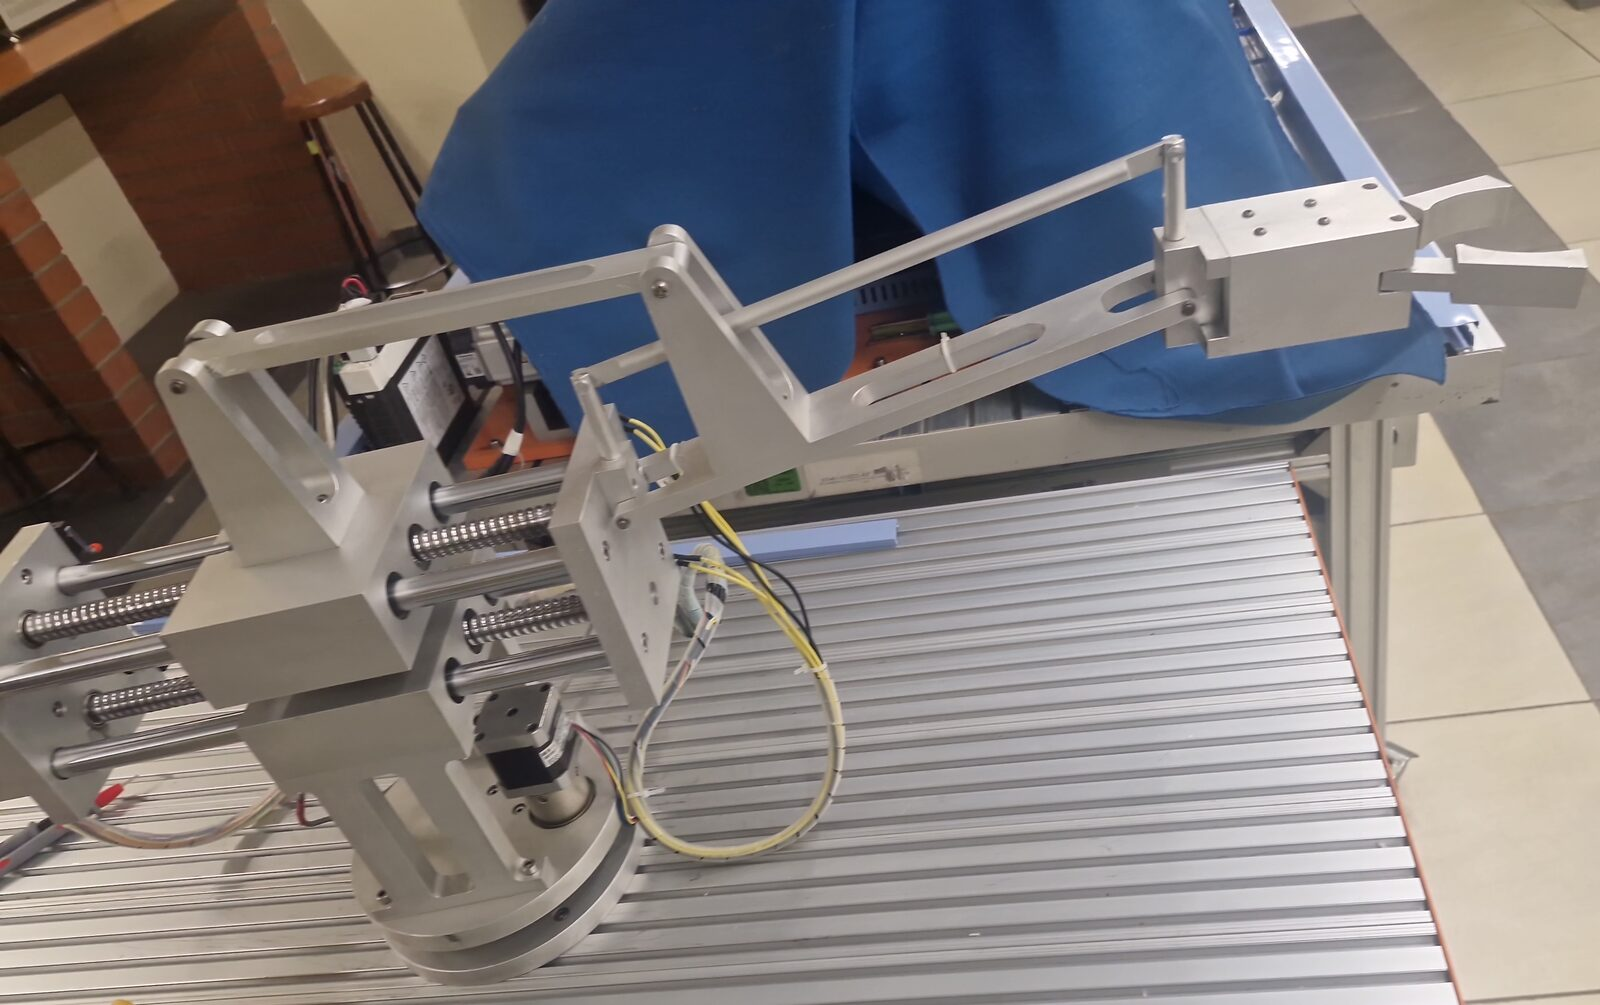
\includegraphics[height=6.5cm, width=0.9\linewidth, keepaspectratio]{brazo_vista_general.jpg}
\caption{Vista general del brazo XK-JS1-1.}
\end{figure}

%======================================================================
\section{ETN-1034: inspección del procesamiento y ficha técnica}
%======================================================================
\subsection{CPU y módulos}
El tablero tiene una sola CPU, \textbf{Siemens S7-200 CPU 224 CN DC/DC/DC} (referencia 6ES7 214-1AD23-0XB8), \textbf{sin módulos de expansión}: no hay módulo analógico EM 231 ni módulos digitales adicionales, de modo que todas las señales de la planta son discretas. Sus datos de catálogo son:
\begin{itemize}
\item alimentación de 24~V DC (rango admisible de 20,4 a 28,8~V);
\item 14 entradas digitales de 24~V DC en dos grupos con común propio (1M para I0.0--I0.7 y 2M para I1.0--I1.5);
\item 10 salidas digitales a transistor de 24~V DC, hasta 0,75~A por punto, en dos grupos (1L+/1M y 2L+/2M);
\item dos salidas de pulsos de alta velocidad, Q0.0 y Q0.1, con generador PTO de hasta 20~kHz;
\item puerto 0 RS-485 con protocolo PPI, para la programación con STEP 7-Micro/WIN y la comunicación con una PC.
\end{itemize}
\begin{figure}[H]\centering
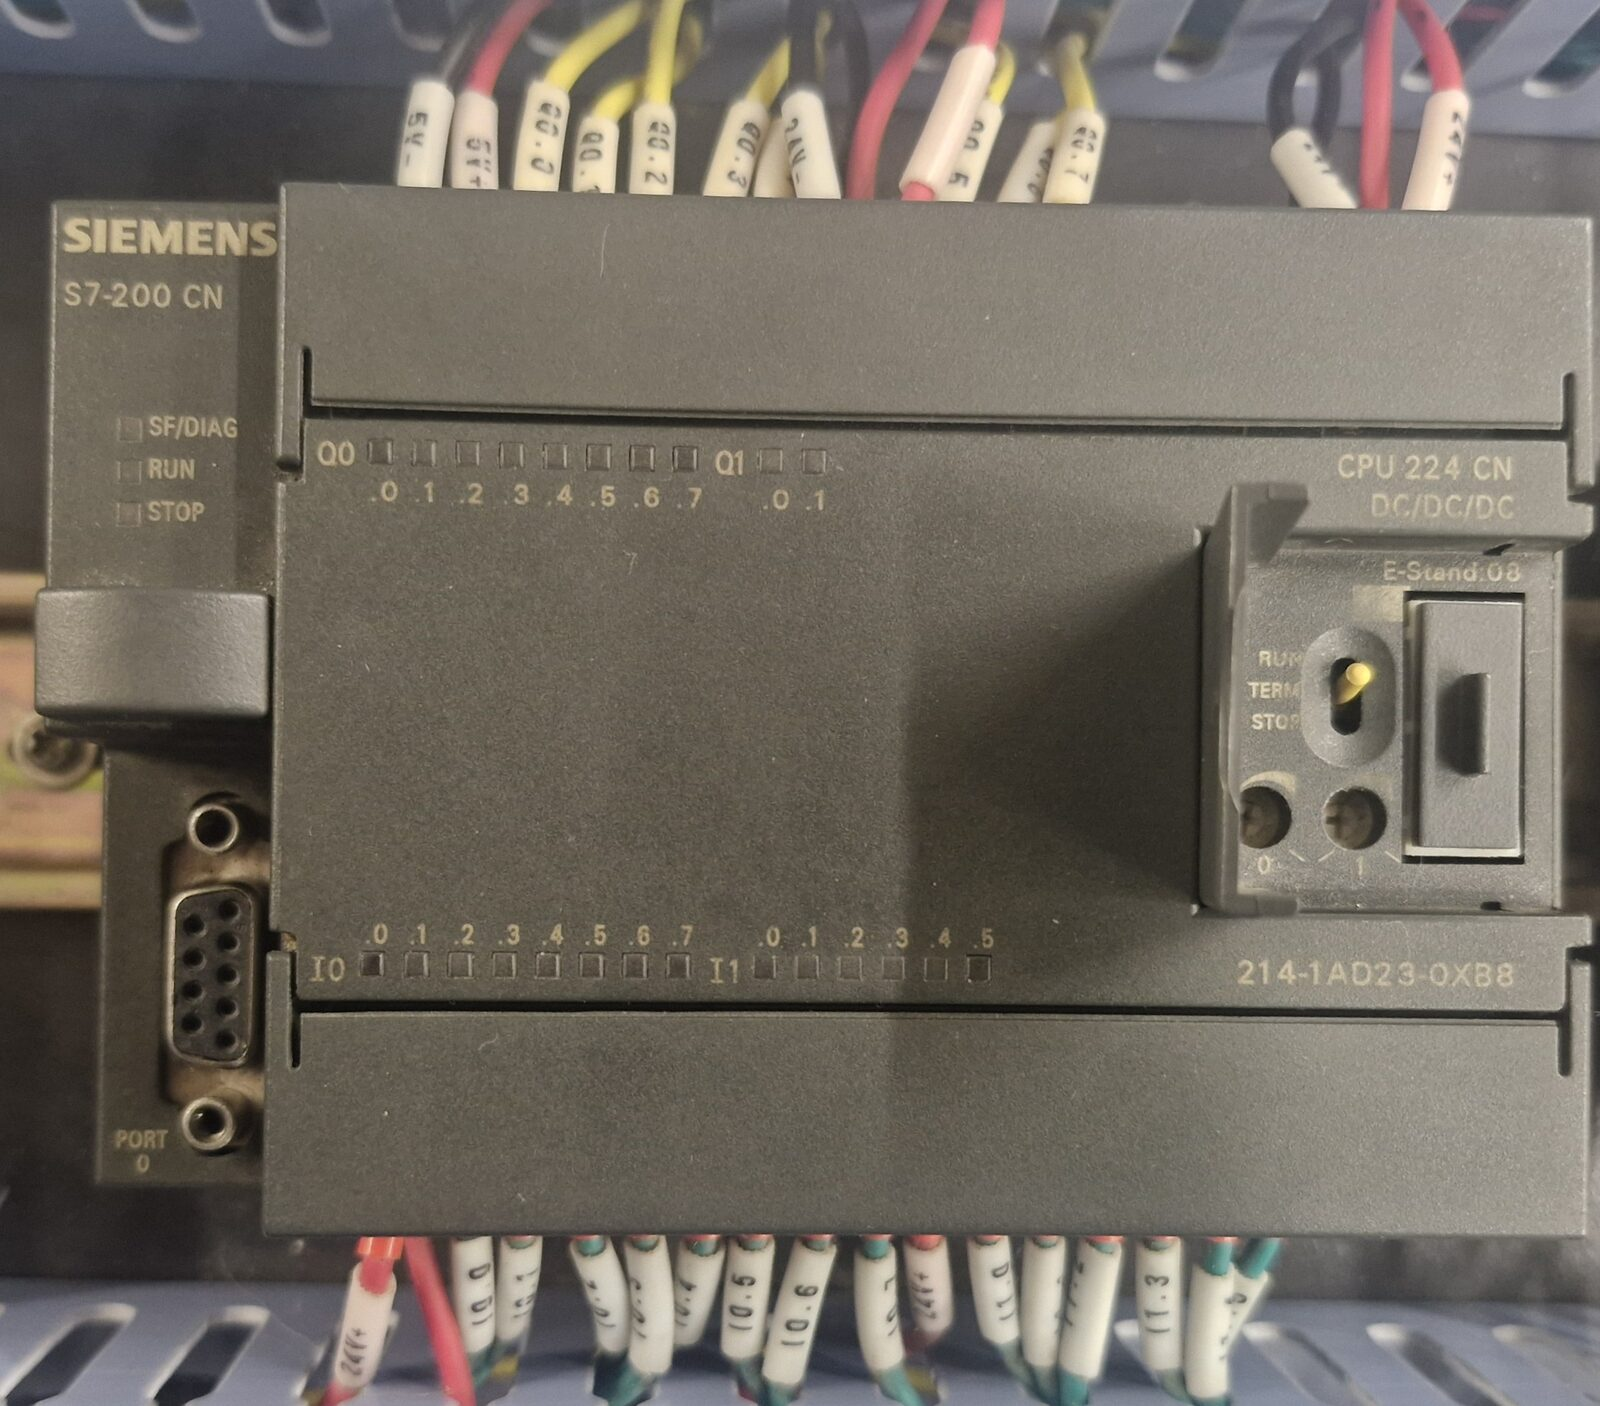
\includegraphics[height=6cm, width=0.8\linewidth, keepaspectratio]{plc_s7-200_cpu224.jpg}
\caption{CPU S7-200 CPU 224 CN del tablero.}
\end{figure}

\subsection{Ficha técnica unificada}\label{sec:ficha}
\begin{center}\small
\begin{longtable}{>{\raggedright}p{2.6cm} >{\raggedright}p{3.6cm} >{\raggedright}p{2.4cm} >{\raggedright\arraybackslash}p{5.6cm}}
\toprule
\textbf{Equipo} & \textbf{Marca / modelo} & \textbf{Tipo de señal} & \textbf{Rango eléctrico y función}\\
\midrule\endhead
Protección general & Disyuntor diferencial DZ47LE-63, curva C & -- & 16~A, 230/400~V AC, fuga 30~mA; protege la entrada de 220~V\\
Fuente & Fuente conmutada & -- & entrada 220~V AC; salidas 24~V DC y 5~V DC para PLC, drivers, relés y sensores\\
Controlador & Siemens S7-200 CPU 224 CN DC/DC/DC & digital 24~V & 14 DI / 10 DO a transistor; PTO en Q0.0 y Q0.1\\
Driver de X e Y & 2M542 (dos unidades) & digital (PUL, DIR, ENA optoacopladas) & 20--50~V DC, 1,0--4,2~A por fase; DIP para 1000 pulsos/vuelta\\
Driver de la base & 2M530 & digital (PUL, DIR, ENA optoacopladas) & 18--50~V DC, 0,5--3,0~A por fase\\
Motores de X e Y & NEMA 23, 57J1854-828 & potencia (bobinas A$\pm$, B$\pm$) & 2,8~A por fase, 1,8° por paso, híbrido bipolar\\
Motor de la base & NEMA 17, 42J1848-604 & potencia (bobinas A$\pm$, B$\pm$) & 1,2~A por fase, 1,8° por paso (200 pasos/vuelta)\\
Relés de selección & Omron MY2N-J 24~V DC (K1 y K2) & digital 24~V & bobina 24~V DC; dos contactos conmutados de 5~A; reparten el tren de pulsos de Q0.1 entre X e Y\\
Finales de carrera & microinterruptores de palanca (4) & digital 24~V & contacto NA/NC, 5~A a 250~V AC; límites y origen de los carros X e Y\\
Sensor de origen de la base & LJ12A3-4-Z/BX & digital NPN, NA & 6--36~V DC, alcance 4~mm, 100~Hz\\
Garra & solenoide de 24~V DC & digital 24~V & accionado directamente por la salida Q0.7\\
Botonera & pulsadores y selectores & digital 24~V & QS (general), QA (manual/automático), Reset, Start, Stop, S1--S7\\
\bottomrule
\end{longtable}\end{center}

\begin{figure}[H]\centering
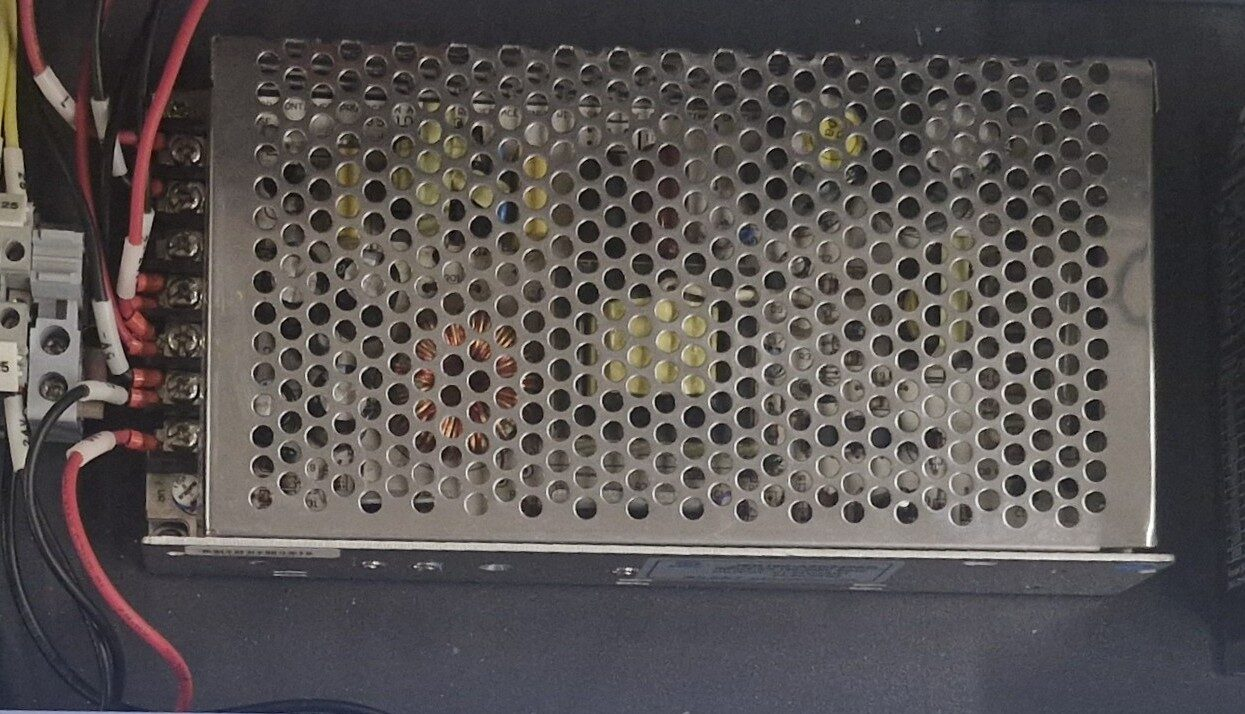
\includegraphics[height=4.2cm, width=0.32\linewidth, keepaspectratio]{fuente_24v_5v.jpg}\hfill
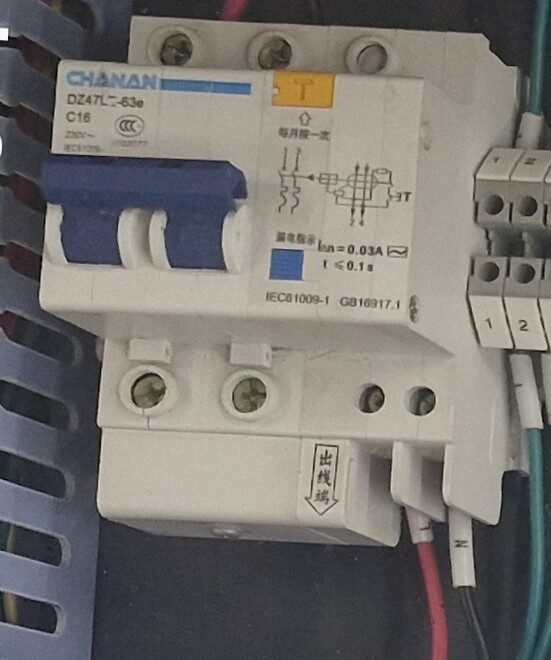
\includegraphics[height=4.2cm, width=0.32\linewidth, keepaspectratio]{disyuntor_dz47le-63.jpg}\hfill
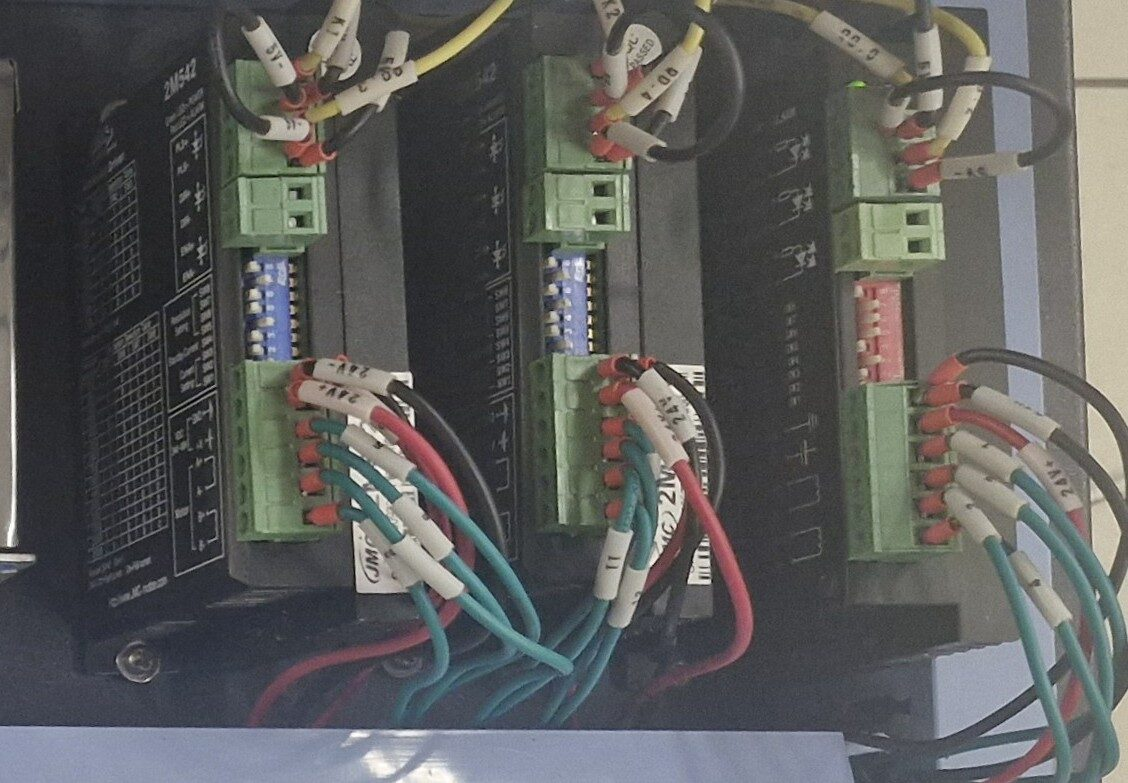
\includegraphics[height=4.2cm, width=0.32\linewidth, keepaspectratio]{drivers_2m542_2m530.jpg}
\caption{Fuente conmutada de 24/5~V (izquierda), disyuntor DZ47LE-63 (centro) y drivers 2M542 y 2M530 (derecha).}
\end{figure}
\begin{figure}[H]\centering
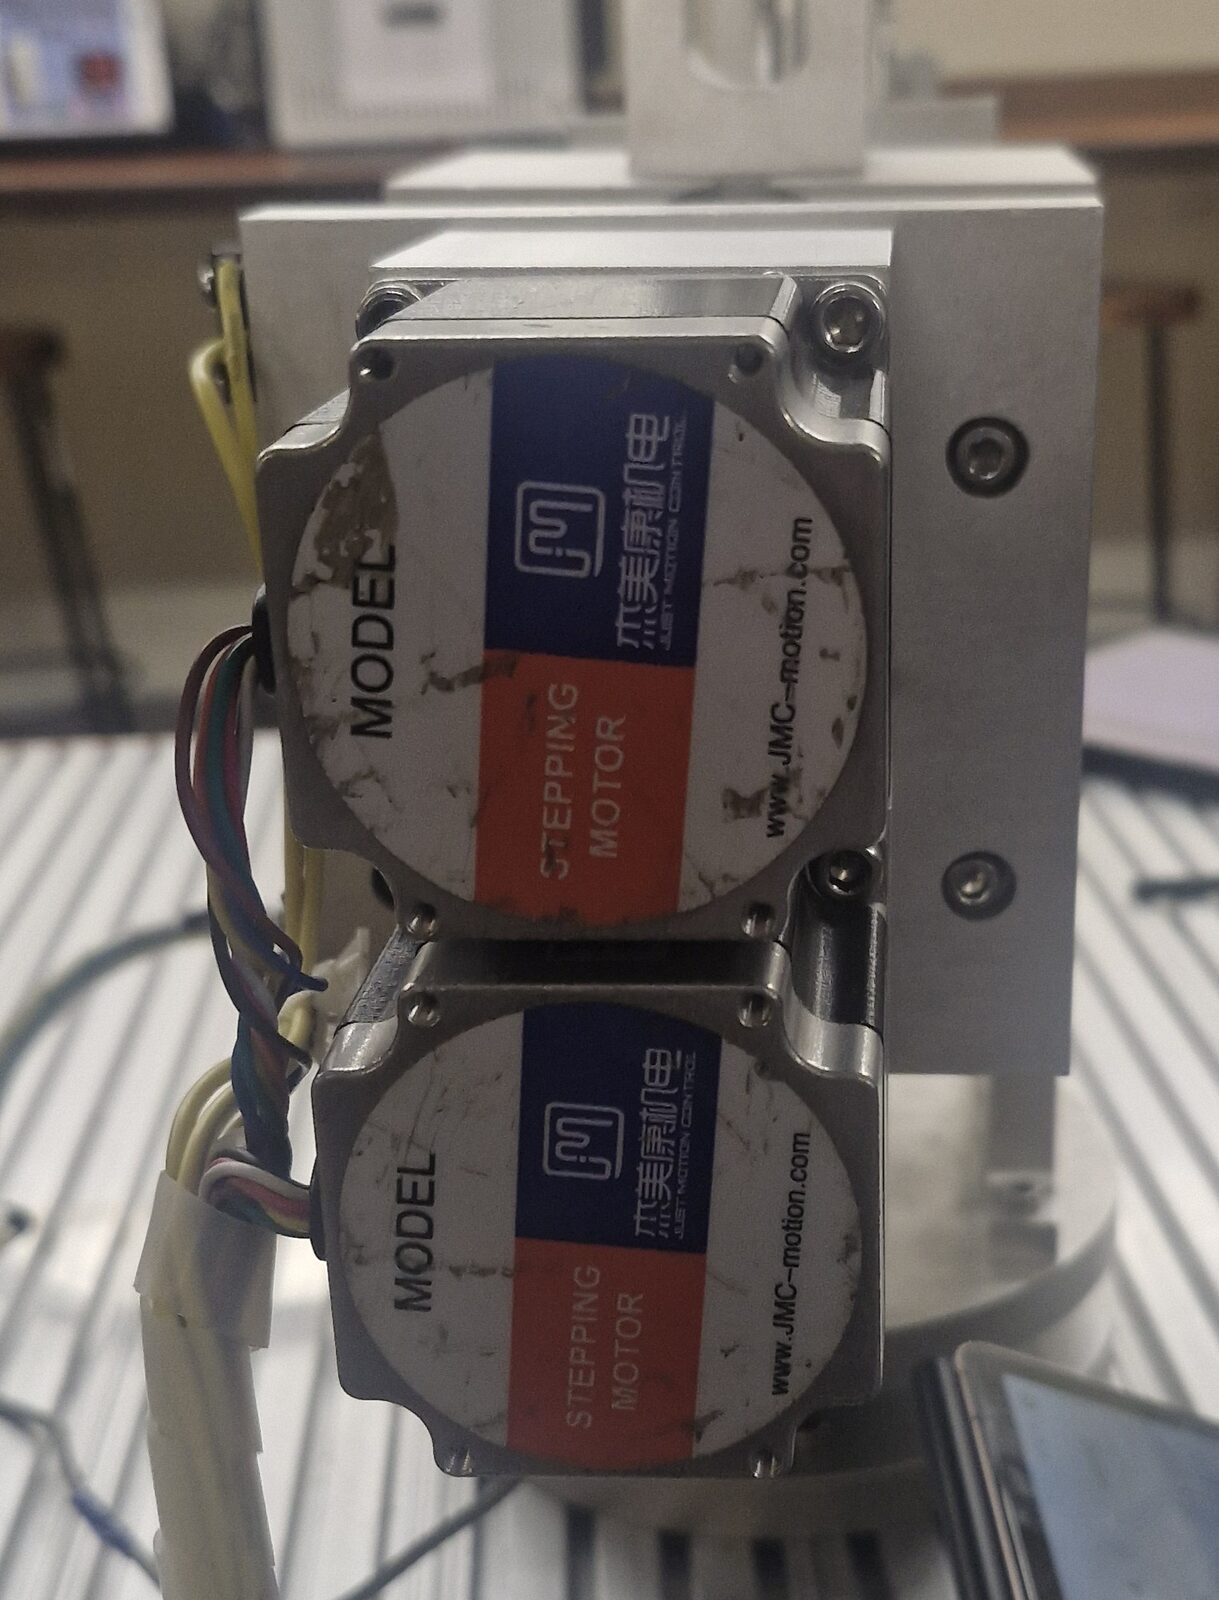
\includegraphics[height=4.2cm, width=0.32\linewidth, keepaspectratio]{motores_nema23_ejes_xy.jpg}\hfill
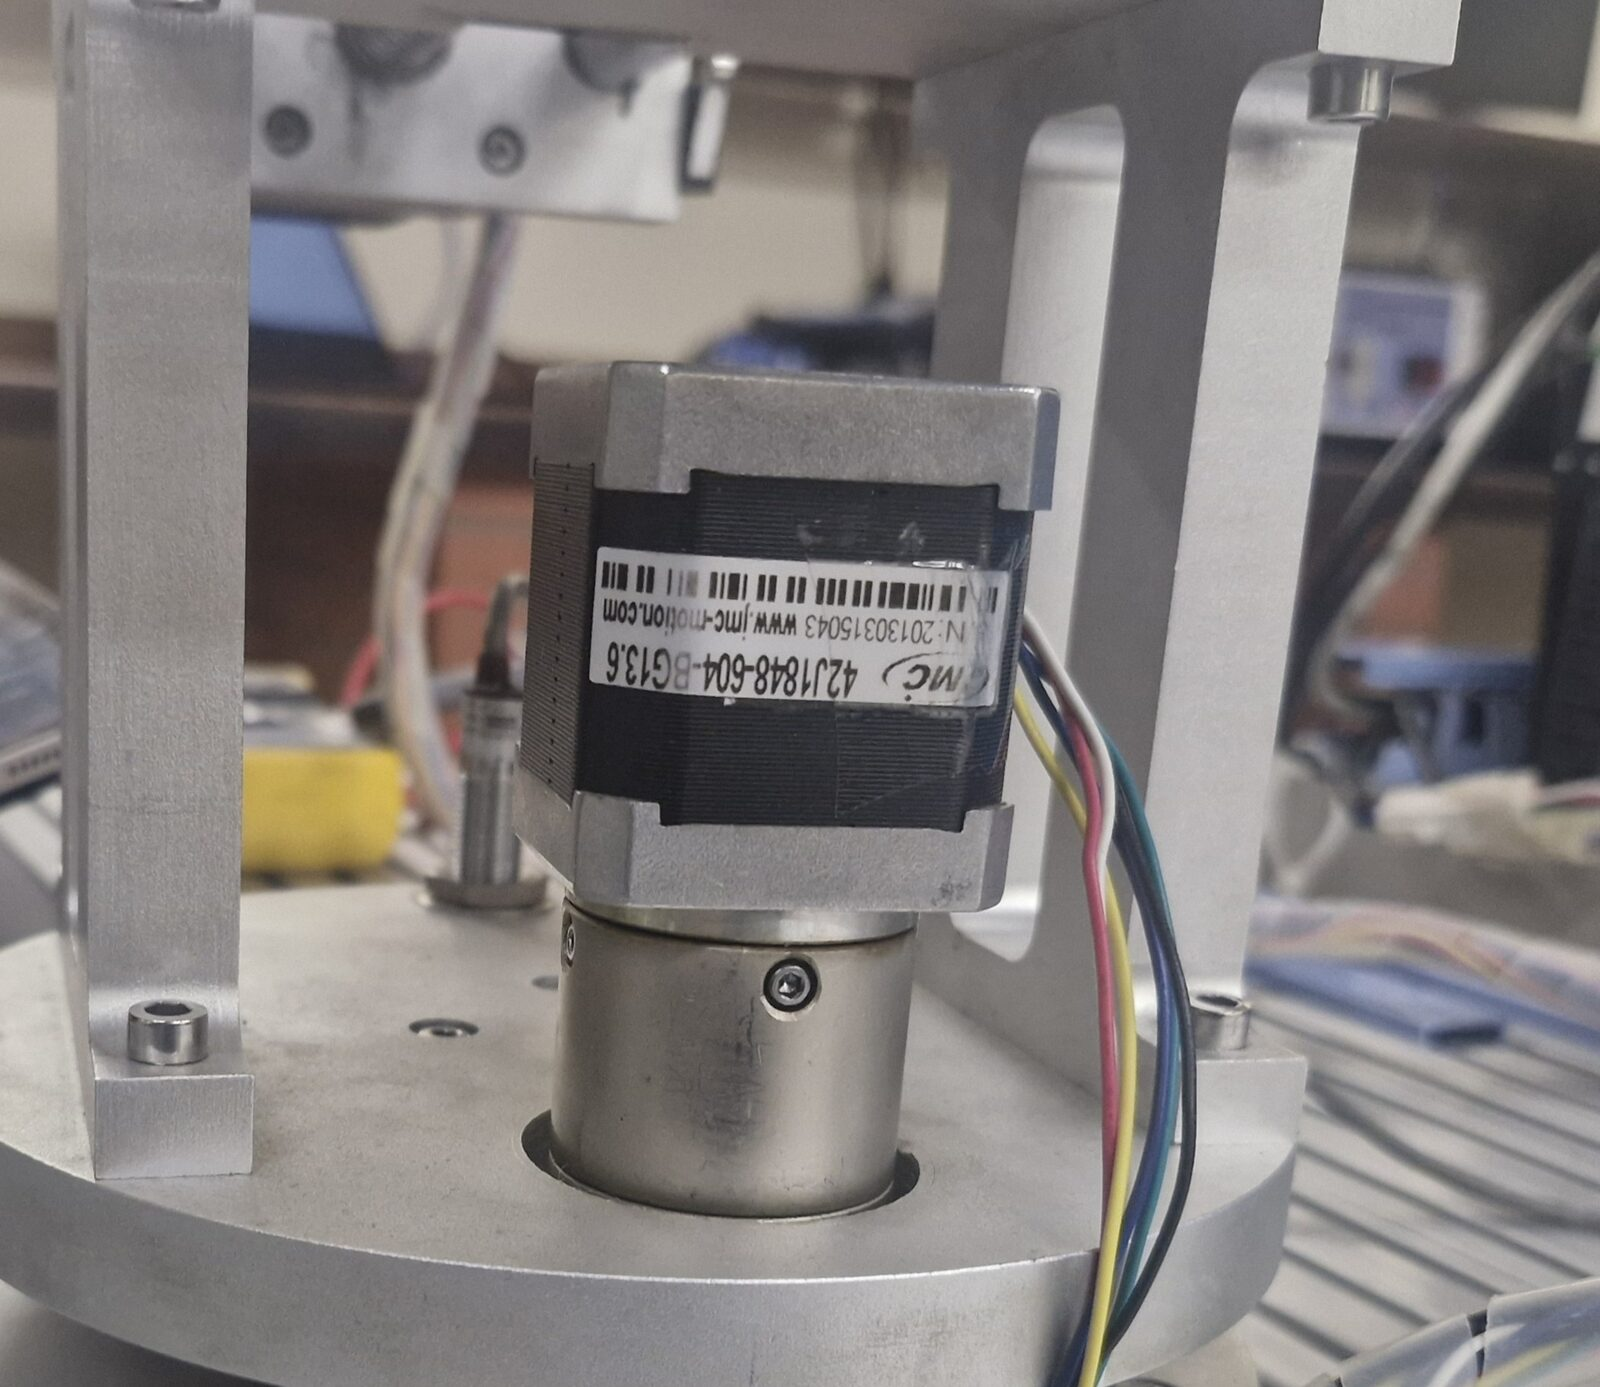
\includegraphics[height=4.2cm, width=0.32\linewidth, keepaspectratio]{motor_nema17_eje_z.jpg}\hfill
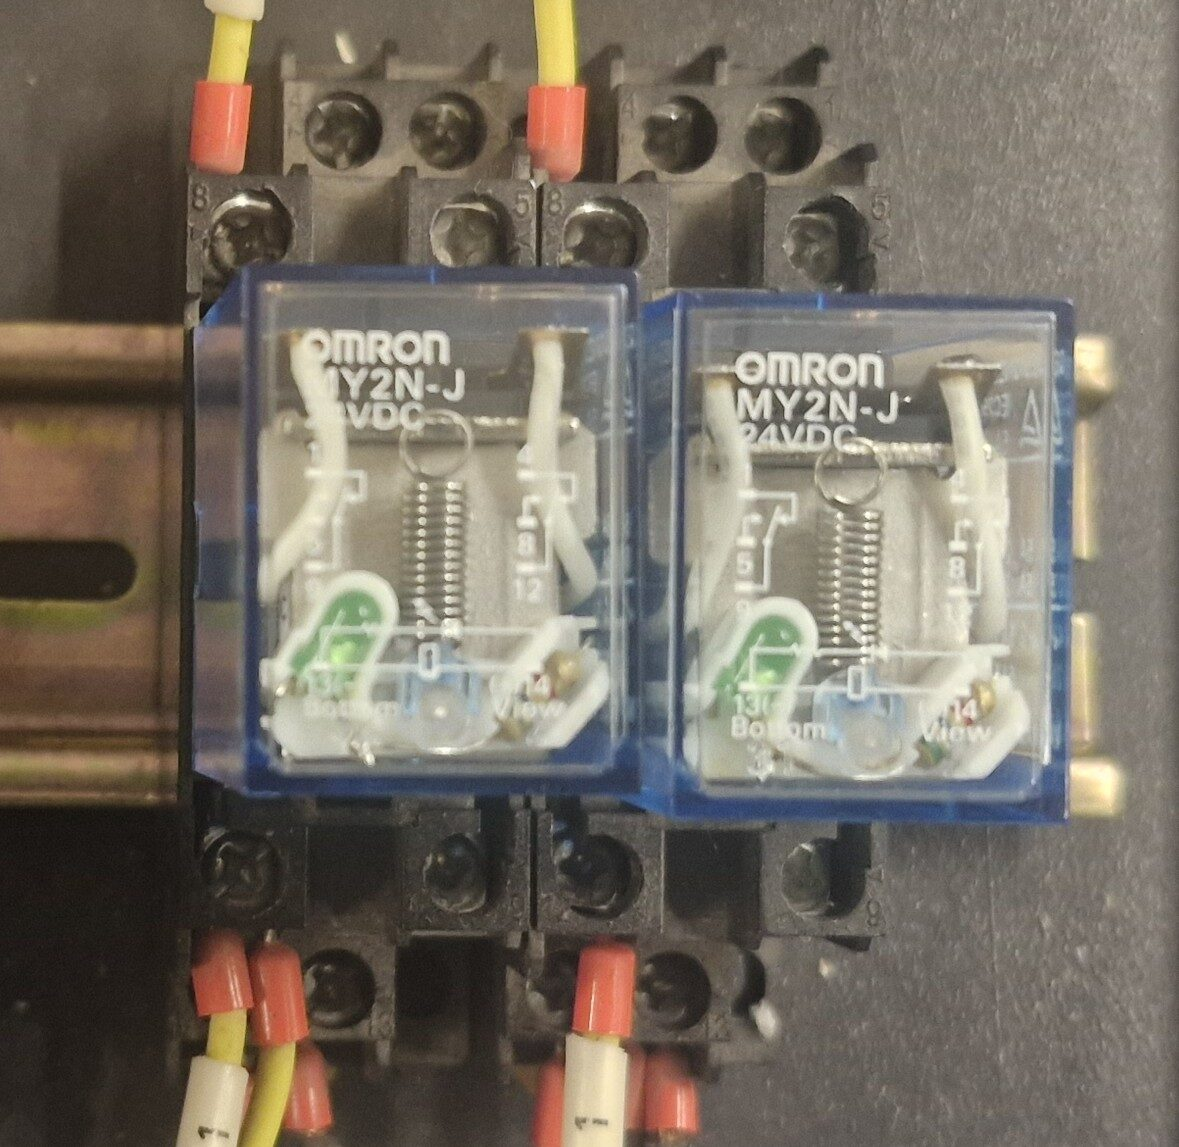
\includegraphics[height=4.2cm, width=0.32\linewidth, keepaspectratio]{reles_omron_my2nj.jpg}
\caption{Motores NEMA 23 de X e Y (izquierda), motor NEMA 17 de la base (centro) y los dos relés Omron MY2N-J (derecha).}
\end{figure}
\begin{figure}[H]\centering
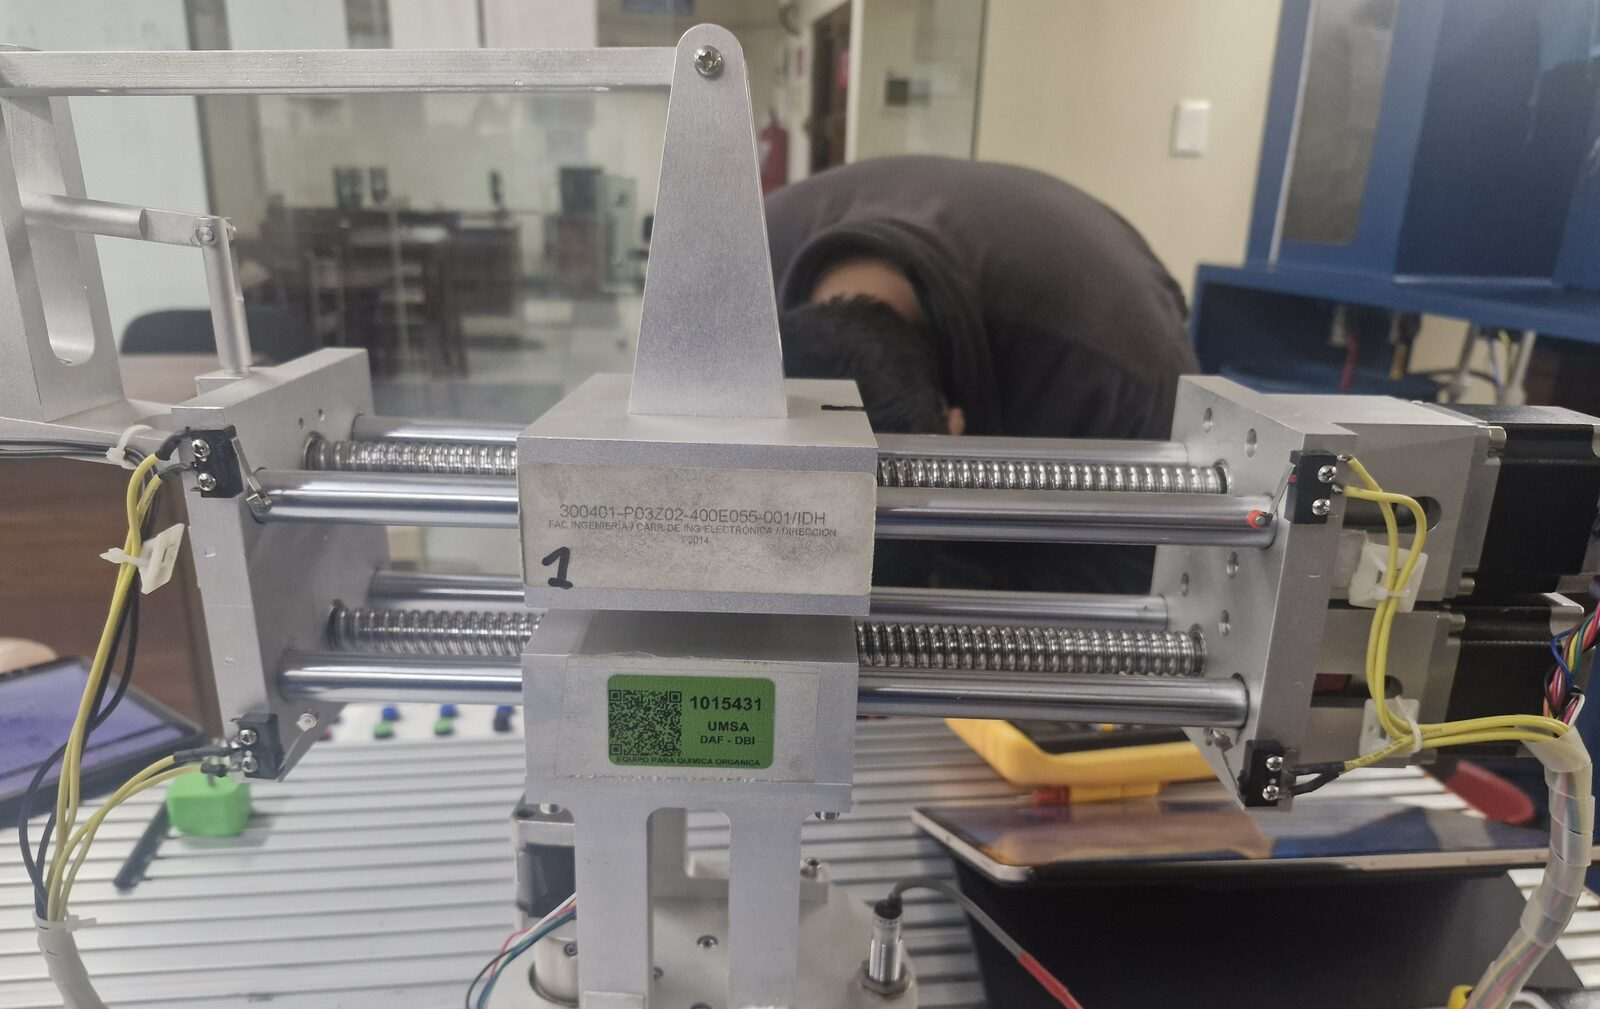
\includegraphics[height=4.2cm, width=0.32\linewidth, keepaspectratio]{final_de_carrera_rieles_xy.jpg}\hfill
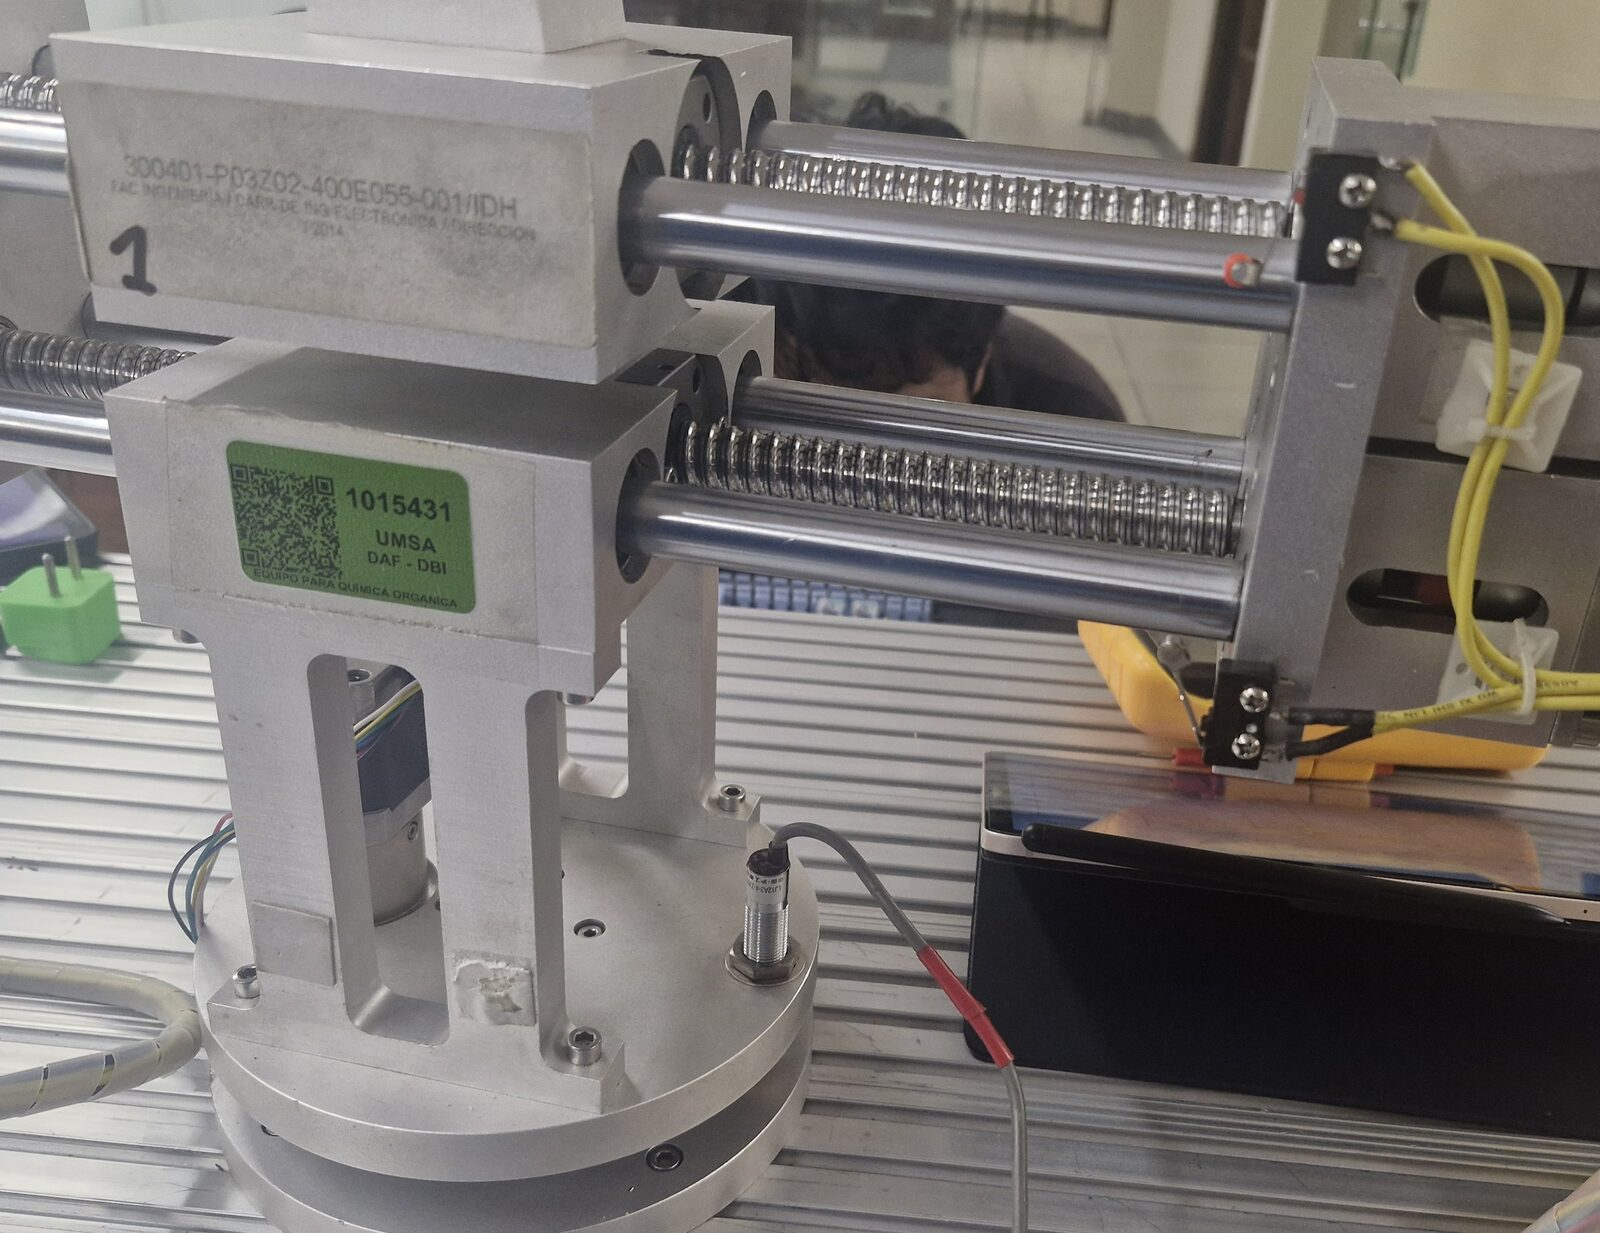
\includegraphics[height=4.2cm, width=0.32\linewidth, keepaspectratio]{eje_z_sensor_inductivo.jpg}\hfill
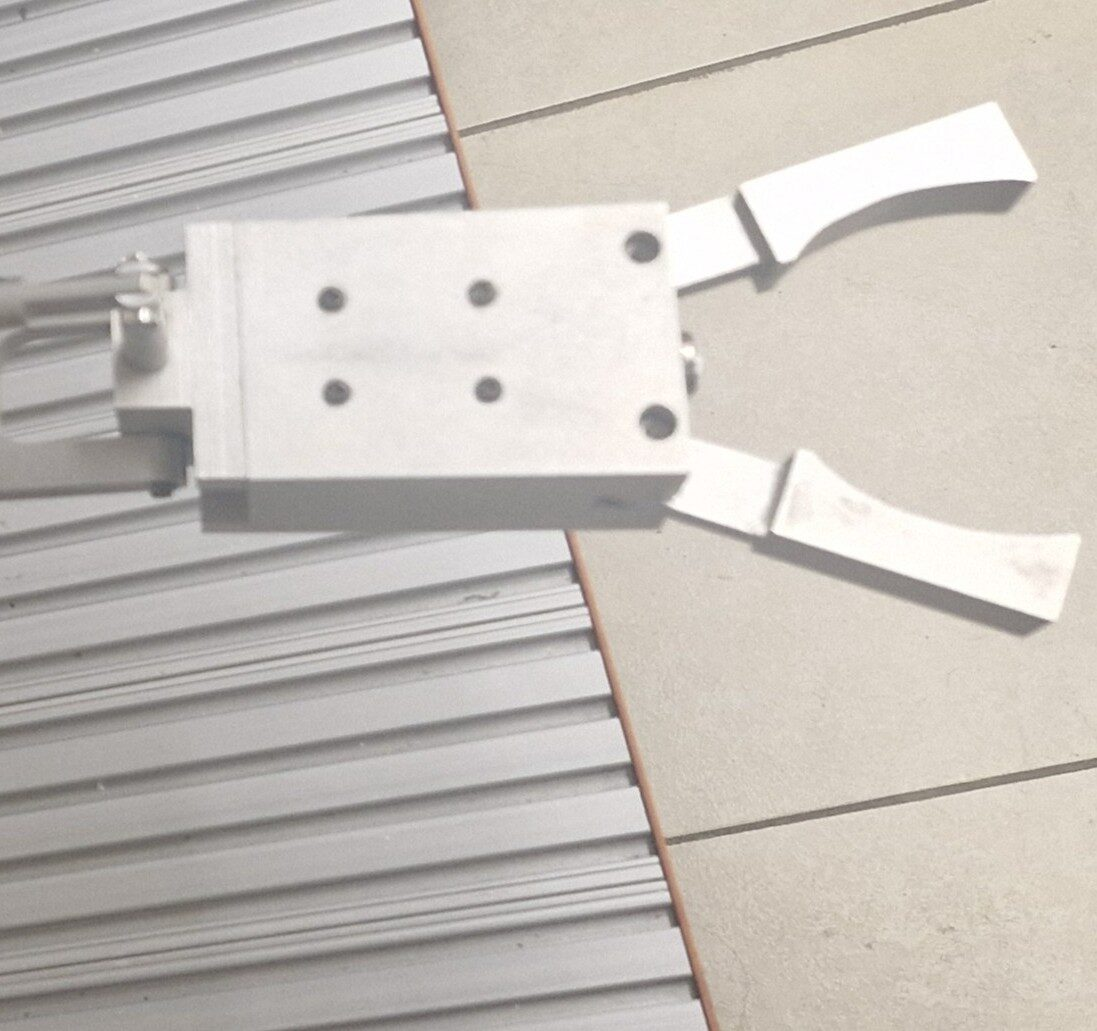
\includegraphics[height=4.2cm, width=0.32\linewidth, keepaspectratio]{garra_solenoide.jpg}
\caption{Finales de carrera de los carros (izquierda), sensor inductivo de la base (centro) y garra de solenoide (derecha).}
\end{figure}
\begin{figure}[H]\centering
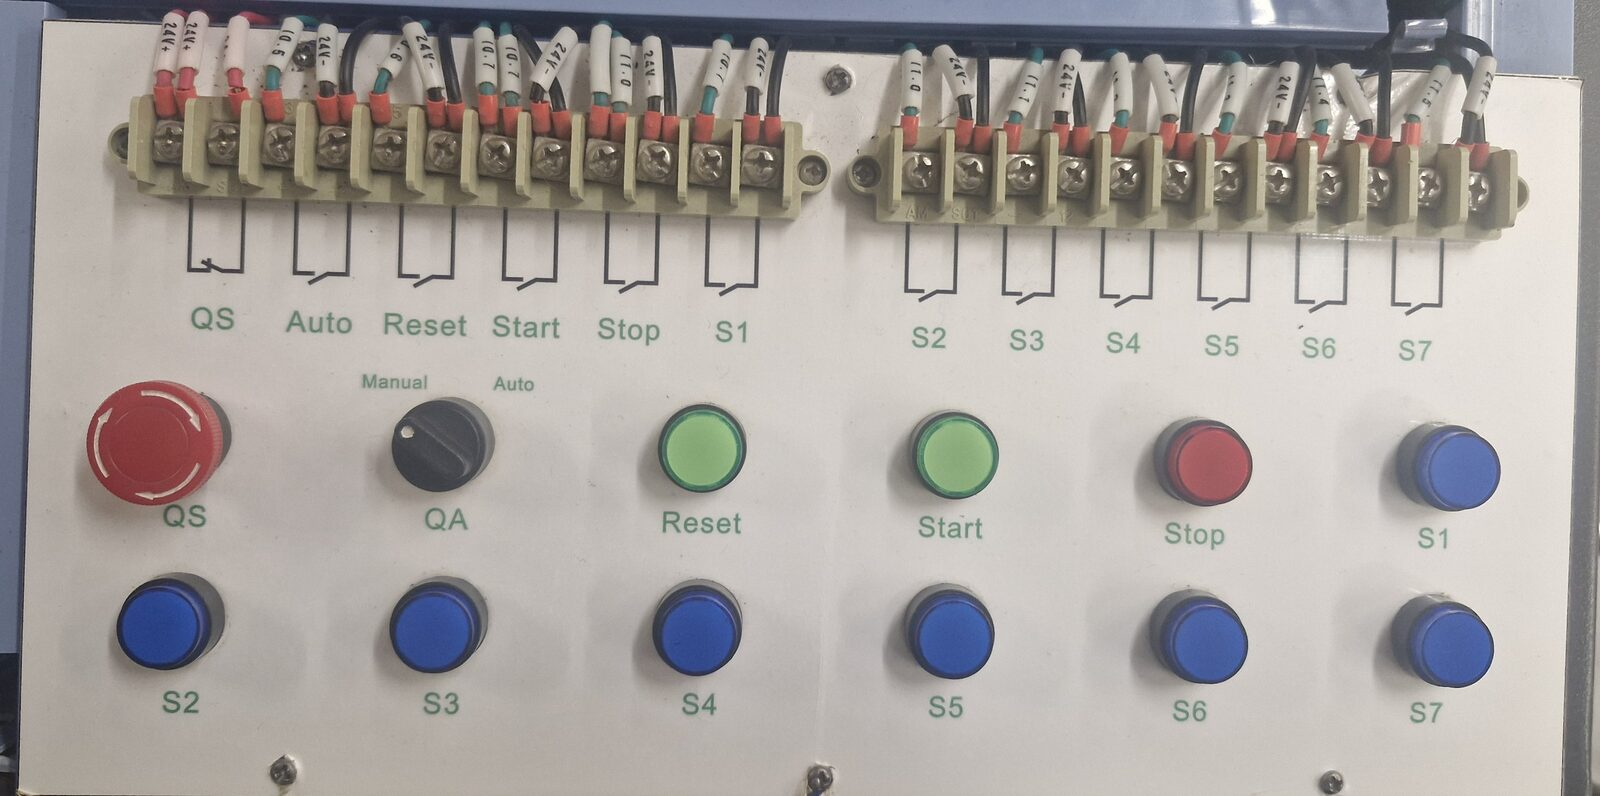
\includegraphics[height=4.5cm, width=0.6\linewidth, keepaspectratio]{botonera.jpg}
\caption{Botonera de operación.}
\end{figure}

%======================================================================
\section{ETN-902: auditoría estática y reporte de discrepancias}
%======================================================================
\subsection{Plano histórico}
Se recibió el plano eléctrico de la gestión anterior y se recorrió la planta cable por cable, verificando con el multímetro la continuidad entre cada borne del PLC, los drivers, los relés y los dispositivos de campo.
\begin{figure}[H]\centering
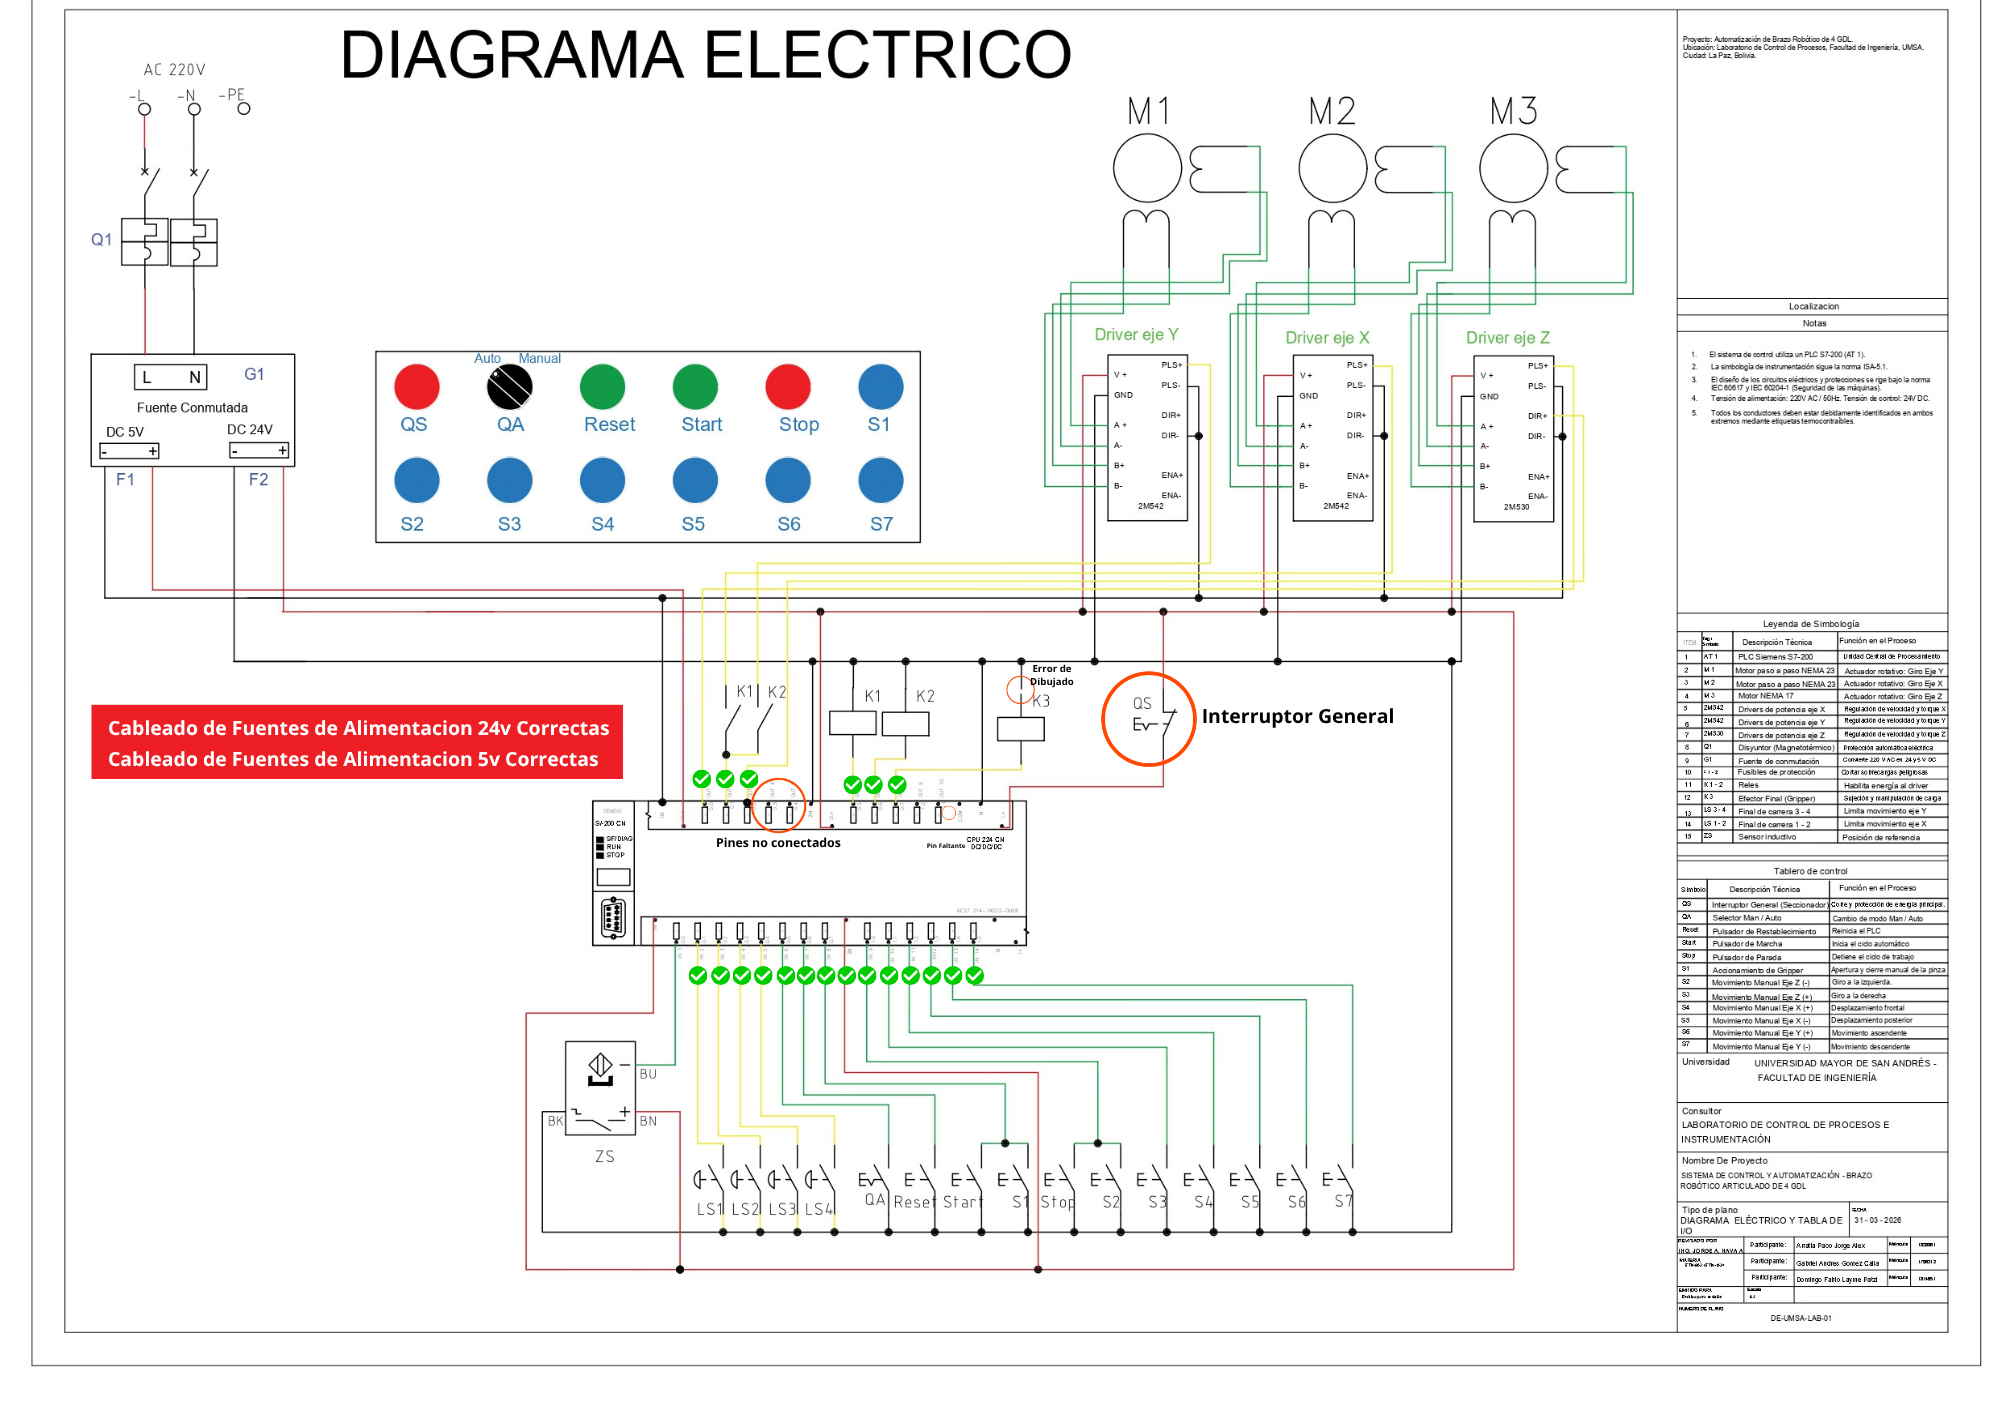
\includegraphics[width=\linewidth]{figuras/plano_historico.png}
\caption{Plano eléctrico histórico, con las marcas de la auditoría.}
\end{figure}
\begin{figure}[H]\centering
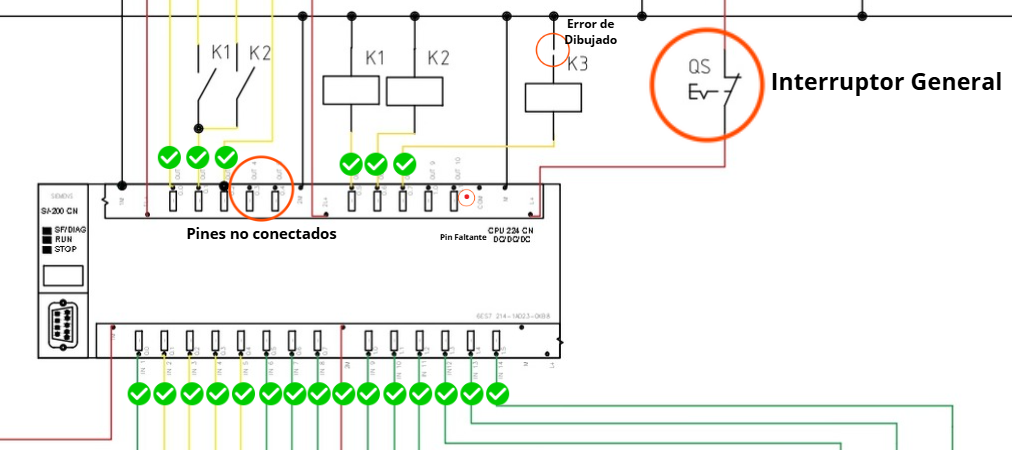
\includegraphics[width=0.49\linewidth]{figuras/historico_pines_plc.png}\hfill
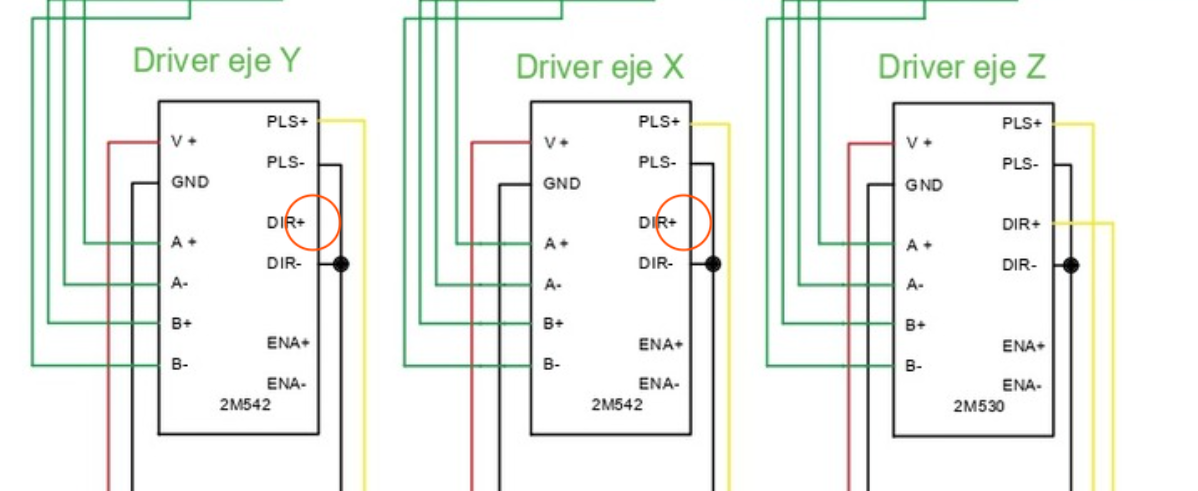
\includegraphics[width=0.49\linewidth]{figuras/historico_dir_drivers.png}
\caption{Detalle de los errores: bornes del PLC sin dibujar y el ``K3'' marcado como error de dibujo (izquierda); entradas DIR+ de los drivers de X e Y sin conexión (derecha).}
\end{figure}

\subsection{Reporte de discrepancias Kaizen}\label{sec:discrepancias}
\begin{center}\small
\begin{longtable}{c >{\raggedright}p{2.8cm} >{\raggedright}p{4.6cm} >{\raggedright\arraybackslash}p{5.6cm}}
\toprule
\textbf{Nº} & \textbf{Elemento} & \textbf{Plano histórico} & \textbf{Planta real (verificado)}\\
\midrule\endhead
1 & Bornes de E/S del PLC & varios bornes de entrada y salida sin dibujar & los bornes existen y están cableados; se verificaron por continuidad\\
2 & Garra & la bobina del solenoide figura como un relé ``K3'' & no hay tercer relé: la salida Q0.7 acciona directamente el solenoide de 24~V de la garra\\
3 & DIR+ del driver de X & entrada sin conexión & conectada a Q0.3 y funcional\\
4 & DIR+ del driver de Y & entrada sin conexión & conectada a Q0.4 y funcional\\
5 & Finales de carrera LS1--LS4 & en I0.0--I0.3 & en I0.1--I0.4 (desfase de un bit); I0.0 es el sensor inductivo de la base\\
6 & Pulsos de X e Y & no se indica cómo se reparten & una sola salida PTO (Q0.1) llega a los dos drivers a través de los contactos de K1 (Q0.5) y K2 (Q0.6)\\
7 & Realimentación de posición & no se declara la ausencia de sensores continuos & no hay encoders en ningún eje: la planta opera en lazo abierto con supervisión discreta (sección~\ref{sec:ruptura})\\
\bottomrule
\end{longtable}\end{center}
Las discrepancias 1 a 6 son requerimientos de corrección para la versión 2.0 de los planos (laboratorio 2); la 7 condiciona toda la estrategia de control de las fases siguientes.

\subsection{Mapeo de variables y vector multifase}
Las señales se midieron de forma pasiva con el multímetro en los bornes del tablero, con la acción presente y en reposo. El multímetro muestra el valor medio, por eso los trenes de pulsos aparecen como tensiones bajas.
\begin{center}\footnotesize
\begin{longtable}{>{\raggedright}p{1.9cm} >{\raggedright}p{2.2cm} >{\raggedright}p{2.6cm} >{\raggedright}p{1.5cm} c c >{\raggedright\arraybackslash}p{2.3cm}}
\toprule
\textbf{Etapa} & \textbf{Variable} & \textbf{Punto físico} & \textbf{Señal} & \textbf{Con acción} & \textbf{En reposo} & \textbf{Observación}\\
\midrule\endhead
Referencia $r(t)$ & mando de botonera & QA, Reset, Start, Stop, S1--S7 (I0.5--I1.5) & digital 24~V & 21,6~V & 23,1~V & entradas del PLC\\
Control $N_p, f_p$ & tren de pulsos & Q0.1 (X, Y por K1/K2), Q0.0 (base) & pulsos & 0,0--1,2~V & 0,1--0,2~V & valor medio\\
Control $\vec D$ & dirección & Q0.3 (X), Q0.4 (Y), Q0.2 (base) & digital & 0,1--5,1~V & 0,1--5,1~V & entrada DIR de los drivers\\
Control $y_G$ & garra & Q0.7 & digital 24~V & 23,2~V & 0,2~V & solenoide energizado\\
Selección & bobinas K1, K2 & Q0.5, Q0.6 & digital 24~V & 0,0~V & 0,0--0,1~V & relés en reposo durante la medición\\
Actuación $i_\varphi$ & corriente de fase & A$\pm$, B$\pm$ & analógica & -- & -- & requiere pinza amperimétrica\\
Planta $\theta, x, y$ & posición & -- & -- & -- & -- & sin encoder: no medible\\
Realim. $s_{FC}$ & finales de carrera & I0.1--I0.4 & digital 24~V & 21,6~V & 23,1~V & desfase de un bit frente al plano\\
Realim. $s_{IND}$ & inductivo de la base & I0.0 & digital NPN & -- & -- & lógica: 0 en el origen\\
Alimentación & rieles de 5~V y 24~V & 1M--1L+, 2M--2L+ & DC & 5,1--23,4~V & 5,2--23,7~V & dentro de rango\\
\bottomrule
\end{longtable}\end{center}

%======================================================================
\section{Análisis de causalidad}
%======================================================================
\subsection{Ruptura de causalidad}\label{sec:ruptura}
El PLC genera pulsos y dirección; los drivers energizan las fases de los motores y el mecanismo se desplaza:
\begin{equation}
u(t) \rightarrow \text{driver} \rightarrow \text{motor} \rightarrow \text{mecanismo} \rightarrow y(t)
\end{equation}
En un control de posición realimentado, un sensor mediría $y(t)$ y el controlador actuaría sobre el error:
\begin{equation}
e(t) = r(t) - y(t), \qquad u(t) = C[e(t)]
\end{equation}
El brazo no tiene encoders ni otro medidor continuo de posición. El PLC solo conoce cuántos pulsos mandó; si cada pulso produce un desplazamiento ideal $\Delta q$, la posición estimada es
\begin{equation}
q_{est} = q_0 + N_p\,\Delta q
\end{equation}
con $q_0$ la posición de referencia (fijada en el homing) y $N_p$ el número de pulsos con su signo de dirección. La fricción en las guías, la variación de la carga, las holguras de la transmisión y la pérdida de pasos hacen que, en general,
\begin{equation}
q_{real} \neq q_{est}
\end{equation}
sin que el PLC pueda medir la diferencia. La cadena de realimentación $y(t) \rightarrow \text{sensor} \rightarrow \text{PLC}$ no existe. Lo único que vuelve al PLC son señales discretas de los finales de carrera y del sensor inductivo,
\begin{equation}
s_i(t) \in \{0, 1\}
\end{equation}
que indican solo si se alcanzó un punto físico concreto. La ruptura de causalidad se resume como
\begin{equation}
u(t) \rightarrow y(t) \quad \text{pero} \quad y(t) \not\rightarrow u(t)
\end{equation}
La acción de control produce efecto sobre la planta, pero ese efecto no vuelve al controlador: el brazo opera en \textbf{lazo abierto con supervisión discreta} y no se puede calcular $e(t)$ en tiempo real.

\subsection{Diagrama de bloques fenomenológico}\label{sec:bloques}
\begin{figure}[H]\centering
\begin{tikzpicture}[x=1cm,y=1cm]
\node[blq=20mm, fill=azulw!8] (op) at (0,0) {Operador\\botonera};
\node[blq=22mm, fill=naranja!12] (plc) at (3.4,0) {Controlador\\PLC S7-200};
\node[blq=20mm] (dx) at (7.4,1.7) {Drivers 2M542\\(X, Y)};
\node[blq=20mm] (db) at (7.4,0) {Driver 2M530\\(base)};
\node[blq=18mm] (mx) at (10.4,1.7) {NEMA 23\\X, Y};
\node[blq=18mm] (mb) at (10.4,0) {NEMA 17\\base};
\node[blq=18mm] (sol) at (10.4,-1.7) {Solenoide\\garra};
\node[blq=18mm, fill=gris] (pl) at (13.4,0) {Planta\\brazo 4 GDL};
\node[blq=26mm, fill=rojo!8] (dv) at (13.4,2.6) {Perturbaciones $d(t)$: fricción, carga, holguras, pasos perdidos};
\node[blq=26mm, fill=verde!10] (sen) at (8.9,-3.3) {Finales de carrera\\sensor inductivo};
\draw[sig] (op) -- node[etiq, above]{$r(t)$} (plc);
\draw[sig] (plc.east) -- ++(0.6,0) coordinate (n) |- (dx.west);
\node[etiq, left] at ($(n)+(0,1.1)$) {$u(t)$: $N_p$, $f_p$, DIR};
\draw[sig] (n) -- (db.west);
\draw[sig] (plc.south east) ++(-0.3,0) |- node[etiq, below, pos=0.8]{Q0.7} (sol.west);
\draw[sig] (dx) -- node[etiq, above]{$i_\varphi$} (mx);
\draw[sig] (db) -- node[etiq, above]{$i_\varphi$} (mb);
\draw[mec] (mx.east) -- ++(0.6,0) |- ($(pl.west)+(0,0.25)$);
\draw[mec] (mb) -- (pl);
\draw[mec] (sol.east) -- ++(0.6,0) |- ($(pl.west)+(0,-0.25)$);
\draw[per] (dv) -- (pl);
\draw[sig] (pl.east) -- ++(0.6,0) node[right, etiq]{$y(t)$};
\draw[dis] (pl.south) |- (sen.east);
\draw[dis] (sen.west) -| node[etiq, below, pos=0.3]{$s_i(t) \in \{0,1\}$} (plc.south);
\end{tikzpicture}
\caption{Diagrama de bloques fenomenológico: lazo abierto con supervisión discreta. Negro: señales de control; gris grueso: acople mecánico; verde discontinuo: realimentación discreta; rojo: perturbaciones. No existe la señal de error $e(t)$.}
\end{figure}

\begin{itemize}
\item \textbf{Referencia $r(t)$}: orden discreta del operador por la botonera (Start, Stop, Reset, S1--S7) o, en automático, la secuencia programada.
\item \textbf{Error $e(t)$}: no existe, porque no hay medición continua de $y(t)$.
\item \textbf{Acción de control $u(t)$}: trenes de pulsos (PTO), dirección y la salida de la garra; es la MV.
\item \textbf{Salida $y(t)$}: posición real de cada eje y estado de la garra; es la PV, pero no se mide de forma continua.
\item \textbf{Realimentación discreta}: finales de carrera y sensor inductivo, solo en puntos fijos (homing y límites).
\end{itemize}

\subsection{Clasificación de variables}
\begin{center}\small
\begin{longtable}{>{\raggedright}p{1.4cm} >{\raggedright}p{4.2cm} >{\raggedright\arraybackslash}p{8.6cm}}
\toprule
\textbf{Tipo} & \textbf{Variable} & \textbf{Descripción y rango}\\
\midrule\endhead
MV & tren de pulsos por eje ($N_p$, $f_p$) & Q0.0 (base) y Q0.1 (X o Y, según K1/K2); pulsos de 24~V hasta 20~kHz\\
MV & dirección por eje & Q0.2 (base), Q0.3 (X, 0 = adelante), Q0.4 (Y, 0 = arriba); digital 24~V\\
MV & orden de la garra ($y_G$) & Q0.7, digital 24~V al solenoide\\
PV & posición estimada por eje ($q_{est}$) & no medible directamente; se calcula como $q_0 + N_p\Delta q$\\
PV & estado de la garra & abierta o cerrada; se infiere de Q0.7\\
PV discreta & referencias de posición ($s_{FC}$, $s_{IND}$) & finales de carrera (I0.1--I0.4) y sensor inductivo (I0.0); solo puntos fijos\\
DV & fricción en guías y transmisión & no medible eléctricamente; separa $q_{est}$ de $q_{real}$\\
DV & carga en la garra & depende del objeto sujetado; no instrumentada\\
DV & holguras y pérdida de pasos & error acumulativo no detectable sin realimentación continua\\
\bottomrule
\end{longtable}\end{center}

\section{ETN-1034: mantenimiento preventivo inicial}\label{sec:mantenimiento}
\paragraph{Sensores y conexiones.} La inspección visual de los finales de carrera encontró puntos de conexión débiles. Se resoldaron los conductores afectados y se protegieron con termocontraíble, para asegurar la continuidad y evitar contactos no deseados.
\paragraph{Borneras.} Se revisaron y ajustaron los conductores de las borneras del tablero que tenían sujeción insuficiente, para eliminar falsos contactos y fallas intermitentes.
\paragraph{Mediciones.} Junto con ETN-902 se midieron las señales de los sensores y de las salidas (vector multifase), siguiendo el procedimiento: identificar el elemento, localizar sus conductores, inspeccionar la conexión, medir de forma pasiva, comparar con el estado físico y registrar.
\paragraph{Pruebas funcionales.} Después del mantenimiento el brazo respondió a las órdenes de movimiento y los finales de carrera conmutaron correctamente en las condiciones de prueba. No se observaron fallas en las conexiones intervenidas. Las holguras mecánicas de las transmisiones quedan registradas como perturbación (DV) del sistema.

\begin{center}\small
\begin{tabularx}{\linewidth}{>{\raggedright}p{3cm} >{\raggedright}X >{\raggedright\arraybackslash}p{4.4cm}}
\toprule
\textbf{Actividad} & \textbf{Procedimiento} & \textbf{Resultado}\\
\midrule
Inspección visual & revisión de sensores, conductores y conexiones accesibles & estado general identificado\\
Resoldadura & reparación de conexiones de los finales de carrera & continuidad y firmeza mejoradas\\
Aislamiento & termocontraíble en las zonas intervenidas & uniones protegidas\\
Borneras & ajuste de conductores flojos & sujeción mejorada\\
Mediciones & medición pasiva de señales con ETN-902 & datos para el vector multifase\\
Pruebas funcionales & movimiento de los ejes y conmutación de los finales & funcionamiento correcto\\
\bottomrule
\end{tabularx}\end{center}

%======================================================================
\section{ETN-1000: arquitectura de datos y requerimientos de persistencia}
%======================================================================
\subsection{Esquema de arquitectura de tres capas}\label{sec:arq}
\begin{figure}[H]\centering
\begin{tikzpicture}[x=1cm,y=1cm]
\draw[rounded corners, fill=azulw!5, draw=azulw!50] (0,-2.4) rectangle (4.6,2.2); \node[font=\small\bfseries, azulw] at (2.3,1.85) {Campo y control};
\draw[rounded corners, fill=naranja!6, draw=naranja!50] (5.6,-2.4) rectangle (10.2,2.2); \node[font=\small\bfseries, naranja!80!black] at (7.9,1.85) {Aplicación};
\draw[rounded corners, fill=verde!6, draw=verde!50] (11.2,-2.4) rectangle (15.8,2.2); \node[font=\small\bfseries, verde] at (13.5,1.85) {Datos};
\node[blq=32mm] (s) at (2.3,0.6) {Sensores y botonera\\\tiny señales digitales de 24 V};
\node[blq=32mm, fill=naranja!12] (p) at (2.3,-1.2) {PLC S7-200\\\tiny registros I, Q y memoria V};
\node[blq=34mm] (m) at (7.9,0.6) {Middleware en la PC\\\tiny lectura cíclica, marca de tiempo, validación de órdenes};
\node[blq=34mm] (u) at (7.9,-1.4) {Interfaz HMI y web\\\tiny operación y consulta};
\node[blq=34mm] (b) at (13.5,-0.4) {Motor relacional\\\tiny tablas normalizadas, transacciones ACID};
\draw[sig] (s) -- (p);
\draw[sig, <->] (p.east) -- node[etiq, above, sloped]{PPI / RS-485} (m.west);
\draw[sig, <->] (m) -- (u);
\draw[sig] (m.east) -- node[etiq, above, sloped]{INSERT} (b.west);
\draw[sig] (b.west) ++(0,-0.3) -- node[etiq, below, sloped]{SELECT} (u.east);
\end{tikzpicture}
\caption{Arquitectura cliente--servidor de tres capas para la telemetría del brazo.}
\end{figure}
\begin{enumerate}
\item \textbf{Capa de campo y control.} Los finales de carrera, el sensor inductivo y la botonera entregan señales digitales al PLC, que genera los pulsos y las direcciones de los drivers. La posición es un valor estimado por conteo de pulsos, guardado en la memoria V del PLC; no hay medición continua.
\item \textbf{Capa de aplicación (middleware).} Un servicio en la PC consulta cíclicamente al PLC por el puerto PPI (RS-485), asocia cada valor a su eje y a su punto de E/S, le agrega la marca de tiempo y lo entrega a la interfaz. En sentido inverso recibe las órdenes del operador (iniciar, detener, mover un eje, accionar la garra), valida su formato y las escribe en el PLC. También aplica la seguridad: si detecta una condición anormal (un final de carrera fuera del punto esperado, pérdida de comunicación) detiene el envío de órdenes y genera una alarma.
\item \textbf{Capa de datos.} Un gestor relacional guarda ciclos de operación, órdenes, estados de E/S, posiciones estimadas, alarmas y tiempos de operación. Las transacciones cumplen ACID: atomicidad (un lote de registros se guarda completo o no se guarda), consistencia (los valores respetan rangos y claves), aislamiento (las lecturas de la interfaz no interfieren con las escrituras del middleware) y durabilidad (lo confirmado sobrevive a un corte de energía).
\end{enumerate}

\subsection{Evaluación de la infraestructura local y latencia}
El cuello de botella del sistema es el enlace serie con el PLC, no la PC. En el puerto PPI cada carácter ocupa 11 bits, de modo que a 9600~bit/s un byte tarda 1,15~ms. Una lectura completa (petición de unos 33 bytes, silencio entre tramas, sondeo y respuesta de unos 67 bytes) dura del orden de 155~ms, es decir, unas 6 lecturas por segundo. Esta tasa es suficiente para supervisar posiciones estimadas y estados discretos, que cambian en escalas de décimas de segundo, y la genera un único maestro: los clientes de la interfaz leen el último estado guardado, sin cargar al PLC.

Una PC de escritorio del laboratorio cubre con holgura el middleware y un gestor relacional local (PostgreSQL o MySQL): el volumen es de unas pocas filas por segundo. Por eso el backend se despliega en la misma PC conectada al PLC, sin necesidad de una PC industrial dedicada. Las fuentes de latencia del lado de la planta son el ciclo de barrido del PLC, la conmutación de los relés K1/K2 y la respuesta de los drivers.

\subsection{Levantamiento de requerimientos de persistencia}
A partir de la entrevista con el equipo de control y de la clasificación de variables, los datos se dividen en:
\begin{itemize}
\item \textbf{Persistentes} (se guardan en la base): ciclos de operación con su modo y duración, órdenes enviadas, estados de las entradas y salidas, posiciones estimadas por eje, alarmas (finales de carrera fuera de lugar, paro, pérdida de comunicación) y sesiones de los operadores.
\item \textbf{No persistentes} (solo en memoria durante la ejecución): el valor instantáneo de cada lectura antes de agruparse, el estado de la interfaz y las variables intermedias del middleware.
\end{itemize}

\subsection{Modelo entidad--relación preliminar}
Una \textbf{planta} (el brazo XK-JS1-1) tiene varios \textbf{ejes de movimiento} (base, X, Y y garra), con su tipo de desplazamiento y recorrido, y un conjunto de \textbf{puntos de E/S} del PLC con su dirección física (I0.0, Q0.5\dots), tipo y clase de señal. Sobre la planta se ejecutan \textbf{ciclos de operación} en modo manual o automático. Durante un ciclo se registran \textbf{variables de proceso} (posiciones estimadas y estados de sensores) y \textbf{acciones de control} (pulsos, dirección, garra), cada una asociada a su eje y a su punto de E/S, con valor y marca de tiempo; se generan \textbf{alertas de desborde} con tipo, severidad y eje; y se registran los \textbf{tiempos de operación} de cada movimiento.

\begin{center}\small
\begin{tabularx}{\linewidth}{>{\raggedright}p{3.4cm} >{\raggedright}p{4.6cm} >{\raggedright\arraybackslash}X}
\toprule
\textbf{Entidad} & \textbf{Atributos principales} & \textbf{Relaciones}\\
\midrule
Planta & nombre, tipo & contiene ejes y puntos de E/S\\
Eje de movimiento & tipo de desplazamiento, recorrido & base, X, Y o garra\\
Punto de E/S & dirección física, tipo, clase de señal & origen o destino de variables y acciones\\
Ciclo de operación & modo, inicio, fin & agrupa lecturas, órdenes y alertas\\
Variable de proceso & tipo, valor, unidad, instante & eje y punto de E/S\\
Acción de control & tipo, valor, instante & eje y punto de E/S\\
Alerta de desborde & tipo, descripción, severidad, instante & eje que la originó\\
Tiempo de operación & inicio, fin, duración & movimiento o ciclo completo\\
\bottomrule
\end{tabularx}\end{center}
\begin{figure}[H]\centering
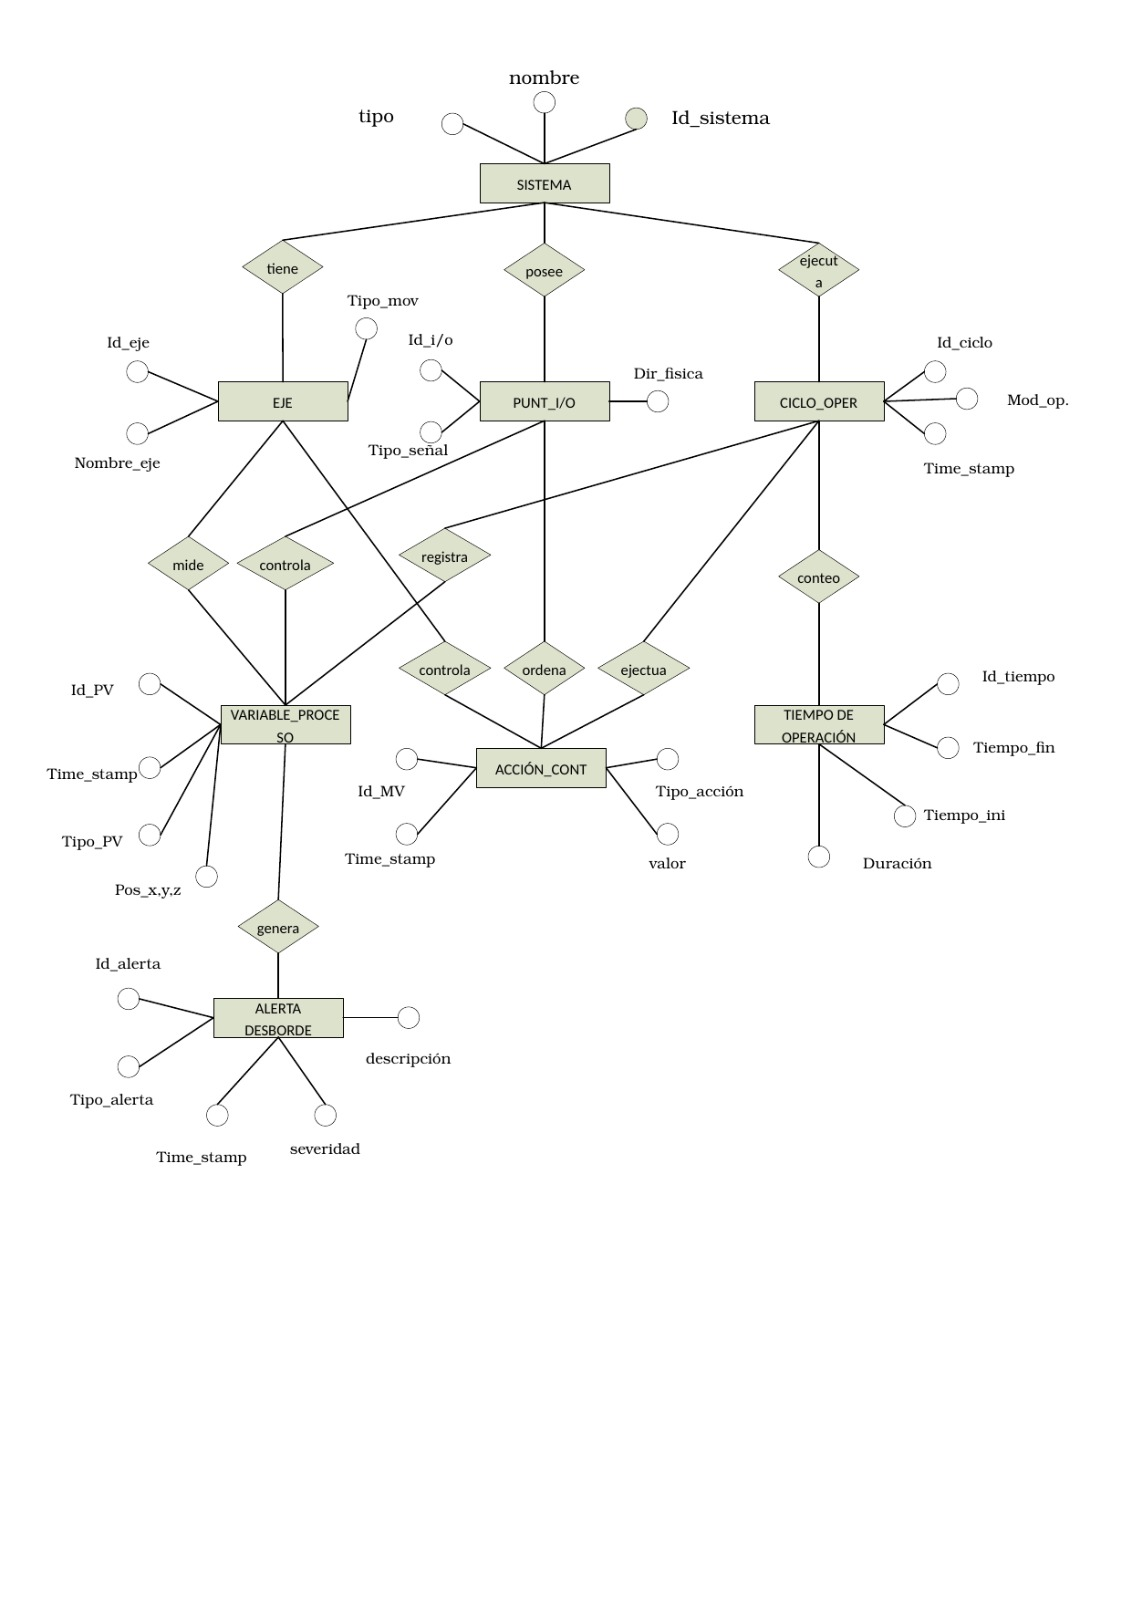
\includegraphics[height=11cm, width=0.75\linewidth, keepaspectratio]{figuras/er_preliminar.png}
\caption{Modelo entidad--relación preliminar (notación de Chen). Se formaliza y normaliza en el laboratorio 3.}
\end{figure}

\section{Entregables (Definition of Done)}
\begin{dod}
Ficha técnica unificada & \cumple & sección~\ref{sec:ficha}: marca, modelo, tipo de señal y rango eléctrico de cada equipo\\
Reporte de discrepancias Kaizen & \cumple & sección~\ref{sec:discrepancias}: siete discrepancias entre el plano histórico y la planta\\
Diagrama de bloques fenomenológico & \cumple & sección~\ref{sec:bloques}, con $r(t)$, $u(t)$, $y(t)$, realimentación discreta y perturbaciones\\
Esquema de arquitectura de datos de 3 capas & \cumple & sección~\ref{sec:arq}\\
\end{dod}

\section{Conclusiones}
\subsection{Equipo de control (ETN-902 / ETN-1034)}
\begin{enumerate}
\item El brazo opera en \textbf{lazo abierto con supervisión discreta}: sin encoders no se puede generar el error $e(t)$ y la posición es una estimación por conteo de pulsos.
\item Por esa razón el sistema es vulnerable a las perturbaciones mecánicas (fricción, carga, holguras): cada paso perdido se convierte en un error de posición acumulativo que el PLC no detecta hasta el siguiente homing.
\item La auditoría encontró siete discrepancias con el plano histórico. Las más graves eran las entradas DIR+ de X e Y dibujadas sin conexión, el desfase de un bit en los finales de carrera y la garra dibujada como un relé ``K3'' inexistente; sin corregirlas la planta no se podría programar ni mantener a partir del plano.
\item El mantenimiento preventivo dejó los sensores y las borneras en buen estado. Para las fases siguientes conviene usar rampas de aceleración en los trenes de pulsos para reducir la pérdida de pasos.
\end{enumerate}
\subsection{Equipo de cómputo (ETN-1000)}
\begin{enumerate}
\item Se clasificaron los datos en persistentes y no persistentes y se identificó el enlace PPI como el factor que limita la tasa de adquisición (unas 6 lecturas por segundo).
\item La posición almacenada será una estimación y así debe registrarse: el modelo la asocia a su eje y a su ciclo para poder auditarla.
\item El modelo E-R preliminar organiza planta, ejes, E/S, ciclos, variables, acciones, alertas y tiempos, y es la base del modelo normalizado del laboratorio 3.
\end{enumerate}

\section*{Bibliografía}
\addcontentsline{toc}{section}{Bibliografía}
\begin{enumerate}[label={[\arabic*]}, leftmargin=*]
\item Nava Amador, J. A. \emph{Guía de Laboratorio Nº 1: auditoría y levantamiento de requerimientos}. ETN-902, ETN-1034, ETN-1000. UMSA, gestión II/2026.
\item Escuadras de la gestión I/2026. Planos y esquemas eléctricos históricos del brazo de 4 GDL. UMSA, Facultad de Ingeniería.
\item ISA. \emph{ANSI/ISA-S5.1-2009: Instrumentation Symbols and Identification}. Research Triangle Park, 2009.
\item Siemens AG. \emph{S7-200 Programmable Controller System Manual}.
\item Siemens AG. \emph{Micro Automation Positioning: biblioteca de posicionamiento por pulsos MAP SERV}, 2010.
\item XK-JS1-1. \emph{Robotic Arm Training Device -- Instruction Book}.
\item Shenzhen Just Motion Control. Manuales de los drivers de motores paso a paso de la serie 2M.
\item OMRON Corporation. \emph{MY Series General-purpose Relays}, hoja de datos.
\item Sensor inductivo LJ12A3-4-Z/BX, hoja de datos.
\end{enumerate}

\end{document}
